%%%%%%%%%%%%%%%%%%%%%%%%%%%%%%%%%%%%%%%%%
% Masters/Doctoral Thesis 
% LaTeX Template
% Version 1.43 (17/5/14)
%
% This template has been downloaded from:
% http://www.LaTeXTemplates.com
%
% Original authors:
% Steven Gunn 
% http://users.ecs.soton.ac.uk/srg/softwaretools/document/templates/
% and
% Sunil Patel
% http://www.sunilpatel.co.uk/thesis-template/
%
% License:
% CC BY-NC-SA 3.0 (http://creativecommons.org/licenses/by-nc-sa/3.0/)
%
% Note:
% Make sure to edit document variables in the Thesis.cls file
%
%%%%%%%%%%%%%%%%%%%%%%%%%%%%%%%%%%%%%%%%%

%----------------------------------------------------------------------------------------
%	PACKAGES AND OTHER DOCUMENT CONFIGURATIONS
%----------------------------------------------------------------------------------------

\documentclass[11pt, oneside]{Thesis} % The default font size and one-sided printing (no margin offsets)

\graphicspath{{Pictures/}} % Specifies the directory where pictures are stored
\usepackage{amsthm}
\theoremstyle{plain}
\newtheorem{thm}{Theorem}[chapter] % reset theorem numbering for each chapter
\theoremstyle{definition}
\newtheorem{defn}[thm]{Definition} % definition numbers are dependent on theorem numbers
\newtheorem{exmp}[thm]{Example} % same for example numbers
\usepackage[all]{xy}
\usepackage{capt-of}
\usepackage{pdfpages}
\usepackage{indentfirst}
\usepackage{textcomp}
\usepackage[square, numbers, comma, sort&compress]{natbib} % Use the natbib reference package - read up on this to edit the reference style; if you want text (e.g. Smith et al., 2012) for the in-text references (instead of numbers), remove 'numbers' 
\hypersetup{urlcolor=blue, colorlinks=true} % Colors hyperlinks in blue - change to black if annoying
\title{\ttitle} % Defines the thesis title - don't touch this

\begin{document}

\frontmatter % Use roman page numbering style (i, ii, iii, iv...) for the pre-content pages

\setstretch{1.3} % Line spacing of 1.3

% Define the page headers using the FancyHdr package and set up for one-sided printing
\fancyhead{} % Clears all page headers and footers
\rhead{\thepage} % Sets the right side header to show the page number
\lhead{} % Clears the left side page header

\pagestyle{fancy} % Finally, use the "fancy" page style to implement the FancyHdr headers

\newcommand{\HRule}{\rule{\linewidth}{0.5mm}} % New command to make the lines in the title page

% PDF meta-data
\hypersetup{pdftitle={\ttitle}}
\hypersetup{pdfsubject=\subjectname}
\hypersetup{pdfauthor=\authornames}
\hypersetup{pdfkeywords=\keywordnames}

%----------------------------------------------------------------------------------------
%	TITLE PAGE
%----------------------------------------------------------------------------------------

\begin{titlepage}
\begin{center}
\HRule \\[0.4cm] % Horizontal line
{\huge \bfseries \ttitle}\\[0.4cm] % Thesis title
\HRule \\[1.5cm] % Horizontal line
\textsc{\Large Master's Thesis}\\[0.5cm] % Thesis type

\large \textit{Submitted in partial fulfillment of the requirement of \\ BITS F421T, Thesis}\\[0.3cm]% University requirement text
\textit{By}\\[0.4cm]
\textbf{\authornames} \\
\textbf{2011B4A3620G} \\
\vspace*{\baselineskip}
Under the Supervision of \\[0.2cm]
\textbf{\supname} \\
Professor of Physics, Department of Physics \\
Fudan University \\ [1cm]

\includegraphics[width=50mm]{BITS_logo.pdf} \\[1cm] % University/department logo - uncomment to place it
\textsc{\LARGE \univname}\\[1.5cm] % University name
{\large \today}\\[4cm] % Date

 
\vfill
\end{center}

\end{titlepage}

%----------------------------------------------------------------------------------------
%	DECLARATION PAGE
%	Your institution may give you a different text to place here
%----------------------------------------------------------------------------------------

\Declaration{

\addtocontents{toc}{\vspace{1em}} % Add a gap in the Contents, for aesthetics
This is to certify that the Thesis entitled, `Boundary conditions of Levin-Wen type models` is submitted by Gangapuram Amit Jamadagni, ID No. 2011B4A3620G
in partial fulfillment of the requirements of BITS F421T Thesis embodies the work done by him under my supervision.

 
Signature of the supervisor:\\
\rule[1em]{25em}{0.5pt} % This prints a line for the signature

Name of the supervisor:\\
\rule[1em]{25em}{0.5pt} % This prints a line for the signature

Date:\\
\rule[1em]{25em}{0.5pt} % This prints a line to write the date
}

\clearpage % Start a new page

%----------------------------------------------------------------------------------------
%	QUOTATION PAGE
%----------------------------------------------------------------------------------------

% \pagestyle{empty} % No headers or footers for the following pages

% \null\vfill % Add some space to move the quote down the page a bit

% \textit{``Something Something"}

% \begin{flushright}
% Dave Barry
% \end{flushright}

% \vfill\vfill\vfill\vfill\vfill\vfill\null % Add some space at the bottom to position the quote just right

%\clearpage % Start a new page

%----------------------------------------------------------------------------------------
%	ABSTRACT PAGE
%----------------------------------------------------------------------------------------

\addtotoc{Abstract} % Add the "Abstract" page entry to the Contents

\abstract{\addtocontents{toc}{\vspace{1em}} % Add a gap in the Contents, for aesthetics

%The Thesis Abstract is written here (and usually kept to just this page). The page is kept centered vertically so can expand into the blank space above the title too\ldots
Topological Phases of Matter at absolute zero cannot be classified by Group theoretical approach. The thesis aims to present the models which classify
these phases of matter and further present various properties of these models. The construction of the  models assumes a lattice structure, with edges and 
nodes being represented in different ways for different models though they form a subclass of the String-Net model by Levin-Wen, according to which the
edges come from a Unitary Tensor Category, the excitations form a Modular Tensor Category. The lattice with boundary is also considered with the boundaries 
given by the modules over algebras of the Modular Tensor Category. The introduction is through the Kitaev Quantum Double Models, the celebrated Toric Code
is one such model, which later are expressed in terms of Categorial parlence. Excitations, along with that condense on the given boundary, are discussed for the 
Quantum Double of $S_{3}$. Ribbon operators which carry excitations at the end are evaluated in the absence and presence of boundaries giving rise to the ribbon operators
which represent anyon condensation in the latter, this leading to the construction of ground states. The identification of boundaries in terms of Category theory is also
presented in terms of theorems. The experience from Quantum Doubles allows one to construct (identifying the boundaries from the theorem) and verify the ground states 
for Ising$\boxtimes$Ising with boundary as Ising, in the absense of ribbon operator. Finally, the construction of ribbon operators analogue, the string operator is presented
with an aim to identify the string operators connecting the bulk to boundary. There has been an extensive use of software tools which include SageMath, Julia, to an extent SymPy
for various calculations.
}

\clearpage % Start a new page

%----------------------------------------------------------------------------------------
%	ACKNOWLEDGEMENTS
%----------------------------------------------------------------------------------------

\setstretch{1.3} % Reset the line-spacing to 1.3 for body text (if it has changed)

\acknowledgements{\addtocontents{toc}{\vspace{1em}} % Add a gap in the Contents, for aesthetics

\setlength{\parindent}{1cm} I would like to thank my mentor, Prof. Ling-Yan Hung, for the wonderful guidance, inspiration, enthusiam and 
valuable insights all along the length of the thesis. I would also like to thank her for giving me an opportunity to
pursue my thesis at Fudan University. I would also like to thank my on-campus supervisior Dr. Prasanna Kumar, for all the inspiration
and support throughout the course. \\

\setlength{\parindent}{1cm} Thanks to my family and friends for the constant support. 
}
\clearpage % Start a new page

%----------------------------------------------------------------------------------------
%	LIST OF CONTENTS/FIGURES/TABLES PAGES
%----------------------------------------------------------------------------------------

\pagestyle{fancy} % The page style headers have been "empty" all this time, now use the "fancy" headers as defined before to bring them back

\lhead{\emph{Contents}} % Set the left side page header to "Contents"
\tableofcontents % Write out the Table of Contents

\lhead{\emph{List of Figures}} % Set the left side page header to "List of Figures"
\listoffigures % Write out the List of Figures

%\lhead{\emph{List of Tables}} % Set the left side page header to "List of Tables"
%\listoftables % Write out the List of Tables

%----------------------------------------------------------------------------------------
%	ABBREVIATIONS
%----------------------------------------------------------------------------------------

\clearpage % Start a new page

\setstretch{1.5} % Set the line spacing to 1.5, this makes the following tables easier to read

\lhead{\emph{Abbreviations}} % Set the left side page header to "Abbreviations"
\listofsymbols{ll} % Include a list of Abbreviations (a table of two columns)
{
% \textbf{LAH} & \textbf{L}ist \textbf{A}bbreviations \textbf{H}ere \\
\textbf{UTC} & \textbf{U}nitary \textbf{T}ensor \textbf{C}ategory \\
\textbf{MTC} & \textbf{M}odular \textbf{T}ensor \textbf{C}ategory \\
\textbf{FC} & \textbf{F}usion \textbf{C}atgory \\
\textbf{RFC} & \textbf{R}ibbon \textbf{F}usion \textbf{C}ategory \\
\textbf{UMTC} & \textbf{U}nitary \textbf{M}odular \textbf{T}ensor \textbf{C}ategory \\
%\textbf{Acronym} & \textbf{W}hat (it) \textbf{S}tands \textbf{F}or \\
}

%----------------------------------------------------------------------------------------
%	PHYSICAL CONSTANTS/OTHER DEFINITIONS
%----------------------------------------------------------------------------------------

% \clearpage % Start a new page

% \lhead{\emph{Physical Constants}} % Set the left side page header to "Physical Constants"

% \listofconstants{lrcl} % Include a list of Physical Constants (a four column table)
% {
% Speed of Light & $c$ & $=$ & $2.997\ 924\ 58\times10^{8}\ \mbox{ms}^{-\mbox{s}}$ (exact)\\
% Constant Name & Symbol & = & Constant Value (with units) \\
% }

%----------------------------------------------------------------------------------------
%	SYMBOLS
%----------------------------------------------------------------------------------------

%\clearpage % Start a new page

%\lhead{\emph{Symbols}} % Set the left side page header to "Symbols"

%\listofnomenclature{lll} % Include a list of Symbols (a three column table)
%{
%$a$ & distance & m \\
%$P$ & power & W (Js$^{-1}$) \\
% Symbol & Name & Unit \\

%& & \\ % Gap to separate the Roman symbols from the Greek

%$\omega$ & angular frequency & rads$^{-1}$ \\
% Symbol & Name & Unit \\
%}

%----------------------------------------------------------------------------------------
%	DEDICATION
%----------------------------------------------------------------------------------------

% \setstretch{1.3} % Return the line spacing back to 1.3

% \pagestyle{empty} % Page style needs to be empty for this page

% \dedicatory{For/Dedicated to/To my\ldots} % Dedication text

% \addtocontents{toc}{\vspace{2em}} % Add a gap in the Contents, for aesthetics

%----------------------------------------------------------------------------------------
%	THESIS CONTENT - CHAPTERS
%----------------------------------------------------------------------------------------

\mainmatter % Begin numeric (1,2,3...) page numbering

\pagestyle{fancy} % Return the page headers back to the "fancy" style

% Include the chapters of the thesis as separate files from the Chapters folder
% Uncomment the lines as you write the chapters

% Chapter 1

\chapter{Mathematical Preliminaries} % Main chapter title

\label{Chapter1} % For referencing the chapter elsewhere, use \ref{Chapter1} 

\lhead{Chapter 1. \emph{Mathematical Preliminaries}} % This is for the header on each page - perhaps a shortened title

%----------------------------------------------------------------------------------------

\section{Category Theory : Definitions and Structures}
 The aim of the section is to provide an overview of the various definitions and formalisms which will be used later in the presentation.
To begin with Linearity, Semisimplicity, Finiteness are defined and then move onto Monoidal Categories,the later sections  
assume Monoidal Categories as a base to introduce other structures like Braiding, Rigidity and Twist, leading to 
the definition of Modularity, leading to Modular Tensor Categories. 

%----------------------------------------------------------------------------------------

\subsection{Linearity, Semisimplicity, Finiteness}

\begin{defn}
Linearity :\\
          A category C is said to be linear, if the Homset(A,B) i.e., the set of morphisms from A to B, $\forall$ A,B $\in$ C forms a vector space over a field of charecteristic zero.
\end{defn}

\begin{defn}
Simple  :\\ 
	An object $x$ $\in$ a category C is said to be simple if $Hom(x,x)$ $\cong$ $C$ (the set of complex numbers). That is the endomorphisms of $x$ is equivalent to $C$. \\
	For further insight refer \citep{Reference15}.
\end{defn}

\begin{defn}
Semisimplicity :\\
          A category C is said to be semisimple, if  every object in C can be written as a direct sum of simple objects in C.
\end{defn}

\begin{defn}
Finite :\\
      A category C is said to be finite, if the number of simple objects in C is finite.
\end{defn}

\subsection{Modular Tensor Categories}
\begin{defn}
Monoidal Category: \\
A category $M$ is said to be monoidal if it is equipped with the following structure :\\
\begin{enumerate}
\item A functor called the tensor product $\otimes$ : $\xymatrix@1{ M\times M}$ $\longrightarrow$ $M$ where $\otimes$ $(x,y)$ = $x$ $\otimes$ $y$ 
   and \\ $\otimes$ $(f,g)$ = $f$ $\otimes$ $g$ $\forall$ objects $x$,$y$ $\in$ $M$ and $\forall$ morphisms $f$,$g$ in $M$ \\
   
\item Natural Isomorphisms called the assosciator:\\
                     \begin{center}
                       $\alpha_{x,y,z} : (x \otimes y) \otimes z \longrightarrow x \otimes (y \otimes z)$
                     \end{center}
         The left unitor:
                     \begin{center}
		      $\beta_{x} : 1 \otimes x \longrightarrow x$
		    \end{center}
         The right unitor:
		    \begin{center}
		     $\gamma_{x} : x \otimes 1 \longrightarrow x$
		    \end{center}
         such that the following diagrams commute. 
                    \begin{center} 
                    $\xymatrix { 
		     &((x \otimes y) \otimes z) \otimes w \ar[dr]^{\alpha_{x \otimes y, w, z}}  \ar[dl]^{\alpha_{x,y,z \otimes 1_{w}}}\\ 
		     (x \otimes (y \otimes z)) \otimes w \ar[d]^{\alpha_{x,y \otimes z, w}}        &          & (x \otimes y) \otimes (z \otimes w) \ar[d]^{\alpha_{x,y,z \otimes w}} \\
		     x \otimes (( y \otimes z) \otimes w) \ar@{-}[r]  &\ar[r]^<(0.05){1_{x} \otimes \alpha_{y,z,w}}   & x \otimes (y \otimes ( z \otimes w))
                    }$  
                       \end{center}
          and 
		    \begin{center}
		    $\xymatrix {
		    (x \otimes 1) \otimes y \ar[dr]^{\gamma_{x} \otimes 1_{y}} \ar@{-}[r] & \ar[r]^<(0.05){\alpha_{x,1,y}}   & x \otimes (1 \otimes y) \ar[dl]^{1_{x} \otimes \beta_{y}}\\
		                                         & x \otimes y     
		    }$
		    \end{center}

\end{enumerate}
\end{defn}

\begin{defn}
Rigidity :\\
      A monoidal category $M$ is said to be rigid, if for each object $A$ $\in$ $M$, $\exists$ an object $A^{*}$ $\in$ $M$ together with the maps : 
      \begin{center}
      $i_{A}$ : $1$ $\rightarrow$ $A$ $\otimes$ $A^{*}$,  \\
      $e_{A}$ : $A^{*}$ $\otimes$ $A$ $\rightarrow$ $1$
      \end{center}
\end{defn}

\begin{defn}
    Fusion Category :\\
	    Fusion category is a finite semisimple C-linear rigid monoidal category such that monoidal unit is simple.
\end{defn}

\begin{defn}
Braided Fusion Category :\\
      A braided fusion category $M$ is a fusion category along with the 
following isomorphisms 
\begin{center}
	  $\xymatrix{
	    \sigma_{x,y} : x \otimes y \longrightarrow^{~} y \otimes x
	   }$
	  \end{center} where $x$, $y$ $\in$ $M$
such that the following diagrams commute.
	\begin{center}
	$\xymatrix{
	x \otimes 1 \ar[r]^{\beta_{x}}  \ar[d]^{\sigma_{1,x}} & x \\
	1 \otimes x \ar[ur]_{\gamma_{x}} &
	}$
      \end{center}
and 
      \begin{center}
      $\xymatrix{
        &x\otimes (y \otimes z) \ar[r]^{\sigma_{x,y \otimes z}} &(y \otimes z) \otimes x \ar[dr]^{\alpha_{y,z,x}} & \\
        (x \otimes y) \otimes z \ar[ur]^{\alpha_{x,y,z}} \ar[dr]^{\sigma_{x,y \otimes 1_{z}}}    & & &y \otimes (z \otimes x) \\
	&(y \otimes x) \otimes z \ar[r]^{\alpha_{x,y,z}} & y \otimes (x \otimes z) \ar[ur]^{1_{y} \otimes \sigma_{x,z}} & 
      }$
      \end{center}
\end{defn}

% \par
% Putting together all the structures until now, we can construct a \emph{Finite Semisimple $C$-Linear Rigid Braided Monoidal Category}. We now define
% a \textit{pivotal structure} on a rigid braided monoidal category, which would be further used in the definition of Ribbon Categories (which are Rigid Braided Monoidal Categoires with a twist).
% \par

\begin{defn}
Pivotial Structure on a fusion category is an isomorphism, \\
\begin{center}
  $\delta_{A}$ : $A$ $\rightarrow$ $A^{**}$ ,such that \\
  $\delta_{A \otimes B}$ = $\delta_{A}$ $\otimes$ $\delta_{B}$ \\
  $\delta_{1}$ = $1$
\end{center}
\end{defn}

\begin{defn}
Ribbon Fusion Category is a Braided Fusion Category with a pivotal structure which is compatible with braiding. 
\begin{center}
  $\theta_{A}$ = $\gamma_{A}$ $\circ$ $\delta_{A}$ : $A$ $\rightarrow$ $A$ via $A^{**}$
\end{center}
\end{defn}

\par
Note : Braided Fusion Category with a pivotal structure is not always a Ribbon Fusion Category, as the pivtoal structure must be compatible with braiding.  
\par

% \begin{defn}
% Ribbon Category :\\
% Ribbon Category is a Rigid Braided Monodial Category with a compatible twist, defined by the isomorphism
% \begin{center}
%  $\theta_{A}$ = $\gamma_{A}$ $\circ$ $\delta_{A}$ : $A$ $\rightarrow$ $A$ via $A^{**}$
% \end{center}
% \end{defn}
\begin{defn}
Spherical Fusion Category : \\
Let $f$ $\in$ $End(X)$ where $X$ is a simple object in $C$ i.e., $f$ : $X$ $\longrightarrow$ $X$ then right trace of the map $f$ is given by
\begin{center}
$Tr^{r}(f)$ = $1$ $\rightarrow$ $x$ $\otimes$ $x^{*}$ $\rightarrow$ $x^{**}$ $\otimes$ $x^{*}$ $\rightarrow$ $x$ $\otimes$ $x^{*}$ $\rightarrow$ $1$
\end{center}
On similar lines,
\begin{center}
$Tr^{l}(f)$ = $1$ $\rightarrow$ $x^{*}$ $\otimes$ $x$ $\rightarrow$ $x^{*}$ $\otimes$ $x^{**}$ $\rightarrow$ $x^{*}$ $\otimes$ $x$ $\rightarrow$ $1$
\end{center}
Fusion Category is said to be spherical if $Tr^{l}(f)$ = $Tr^{r}(f)$ $\forall$ $f$ $\in$ C
\end{defn}

\begin{defn}
Quantum Dimension of an object $X$ in category C is given by $d_{X}$ := $Tr(1_{X})$,
we define $D$ = $\varSigma$ $d_{i}^{2}$
\end{defn}

\begin{defn}
We define the modular matrix S, whose elements are given by
\begin{center}
$s_{ij}$ = $Tr(1_{i \otimes j})$ = $d_{i \otimes j}$, $\forall$ $i$, $j$ $\in$ C
\end{center}
\end{defn}
Finally we define Modular Tensor Category (MTC), 
\begin{defn}
Modular Tensor Category :\\
  MTC is a RFC such that the $det(S)$ $\neq$ $0$.
  
  % MTC is a Finite Semisimple Linear Ribbon category along with the modularity condition, that is the S-matrix is invertible (invariant of the hopf link)
% WIP.
\end{defn}

\subsection{Left, Right Modules over a Category}
We define a left module over a tensor category, this is later used to define the boundaries for the Levin-Wen Models in Chapter \ref{Chapter3}.

\begin{defn}
Left Module Category:\\
      Left Module Category over a monoidal category $C$, is a category $M$ equipped with a $C$ action : a functor $\otimes : C \otimes M \rightarrow M$ such that
there are isomorphisms :
\begin{center}
 $ X \otimes (Y \otimes M') \rightarrow (X \otimes Y) \otimes M' $\\
 $ \textbf{1} \otimes M' \rightarrow M'$
\end{center}
for $X, Y \in C$ and $M' \in M$ satisfying some coherence conditions.
\end{defn}

The definition of Right module is on similar lines.
% \subsection{Graphical Calculus}
 % Graphical Calculus is another way of viewing the objects and morphism space of a Category in terms of graphs. The objects are denoted by strings and the morphisms as nodes.
% For example : A $\otimes$ B $\rightarrow$ C $\otimes$ D. 

% Given objects A,B,C,D,E the basis space construction looks as follows and the conversion between the basis space, given by

% is given by F-Matrix (we refer to this as F-move).

% The unit object and unit morphisms are represented by emptiness.

% Give an example citing the above and also a general representation.

% This would be further used in Chapter 4.


\section{Drinfeld Double of a Group}
    To introduce the Drinfeld Double of a Group, denoted by $D(G)$, we first define Algebras, Co-algebras, Bialgebras and Hopf Algebras.
    
\subsection{Algebras, Co-algebras, Hopf Algebras}
\begin{defn}
Algebra : \\
        Let $A$ be a vector space over a field $K$. The triple $(A, m, \eta)$ is an associative algebra, where

    $m : A \otimes A \rightarrow A$ (multiplication map), \\
    $\eta : K \rightarrow A$ (unit map),\\
such that $m, \eta$ satisfy the following commutation diagrams \\
\begin{center}
$\xymatrix{
A \otimes A \otimes A \ar[r]^{m \circ id_{A}} \ar[d]^{id_{A} \circ m} & A \otimes A \ar[d]^{m} \\
A \otimes A \ar[r]^{m}  & A 
}$
\end{center}
and \\
\begin{center}
$\xymatrix{
A \ar[r]^{id_{A} \circ \eta} \ar[d]^{\eta \circ A} & A \otimes A \ar[d]^{m} \\
A \otimes A \ar[r]^{m}  & A 
}$
\end{center} 
\end{defn}

\begin{defn}
Co-Algebra : \\
        Let $C$ be a vector space over a field $K$. The triple $(C, n, \delta)$ is a co-algebra, where

    $n : C \rightarrow C \otimes C$ (comultiplication map)\\
    $\delta : C \rightarrow K$ (counit map),\\
such that $m, \delta$ satisfy the following commutation diagrams \\
\begin{center}
$\xymatrix{
C \ar[r]^{n} \ar[d]^{n} & C \otimes C \ar[d]^{id_{C} \circ n} \\
C \otimes C \ar[r]^{n \circ id_{C}}  & C \otimes C \otimes C
}$
\end{center}
and \\
\begin{center}
$\xymatrix{
C \ar[r]^{\delta} \ar[d]^{\delta} & C \otimes C \ar[d]^{id_{C} \otimes \delta} \\
C \otimes C \ar[r]^{\delta \otimes id_{C}}  & C 
}$
\end{center} 
\end{defn}

\begin{defn}
Bialgebra : \\
    Let $B$ be a vector space over a field $K$. A quintuple $(B, m, n, \eta, \delta)$ is a bialgebra, where
$(B,m,\eta)$ is an algebra and $(B,n,\delta)$ is a co-algebra.
\end{defn}


\begin{defn}
Hopf Algebra: \\
      Let $H$ be a vector space over a field $K$. The quintuple $(H, m, n, \eta, \delta)$ along with the antipode map $S$
\begin{center}
    $S : H \rightarrow H$ 
\end{center}
such that the following diagram commutes 
\begin{center}
 $\xymatrix{
 H \otimes H \ar[rr]^{id_{H} \otimes S} & & H \otimes H \ar[d]^{m} \\
 H \ar[r]^{\delta} \ar[u]^{n} \ar[d]^{n} & K \ar[r]^{\eta} & H \\
 H \otimes H \ar[rr]^{S \otimes id_{H}} &  & H \otimes H \ar[u]^{m}
 }$
\end{center}
forms a Hopf Algebra.
\end{defn}

\subsection{Drinfeld Double (Quantum Double) of a finite group}
    Let $G$ be a finite group and $K$ be a field. The group algebra $K[G]$ is the set of all linear combinations of elements from $G$ with 
the scalars coming from the field $K$. This forms a vector space and by defining the comultiplication $n(g)$ := $g \otimes g$ and 
counit by $\delta(g)$ = 1, and the antipode $S(g) = g^{-1}$ turns the group algebra $K[G]$ into a Hopf Algebra by the above definitions.

    Let $K(G)$ be the set of functions on $G$ with values in $K$. The basis space is given by $\delta_{g}$ defined by the projection 
$\delta_{g}$(h) = $\delta_{g,h}$. This forms a vector space and is an algebra with point-wise multiplication, with the unit given by
$\eta : K \rightarrow K(G)$ is defined by $\eta(\lambda)(g) = \lambda$, with comultiplication, counit and antipode given by :
\begin{center}
    $(n f)(g,h) = f(gh), \delta(f) = f(e), (Sf)(g) = f(g^{-1})$
\end{center}
Thus, $K(G)$ is a Hopf Algebra using the above definitions.

\begin{defn}
Quantum Double of a group $G$, $D(G)$ : \\
    The vector space $K(G) \otimes K[G]$ along with the following structure :\\
\begin{center}
    $(\delta_{g} \otimes x)(\delta_{h} \otimes y) = \delta_{gx,xh}(\delta_{g} \otimes xy)$,\\
    $ 1 = \sum_{g \in G} \delta_{g} \otimes e$, \\
    $ n (\delta_{g} \otimes x) = \sum_{g_{1}g_{2} = g}(\delta_{g_{1}} \otimes x) \otimes (\delta_{g_{2}} \otimes x)$, \\
    $ \Delta(\delta_{g} \otimes x) = \delta_{g,e}$,\\
    $ S(\delta_{g} \otimes x) = \delta_{x^{-1}g^{-1}x} \otimes x^{-1}$.
\end{center}
\end{defn}
forms a Hopf Algebra, which is defined as Quantum Doulbe of a group $G$, $D(G)$.    

\subsection{Representations of Drinfeld Double of a Group}
    Consider an element $a \in G$ and let $\pi$ be a representation of $Z(a)$ over the vector space $W$ 
with basis $\{w_{1}, ...., w_{d}\}$. Define the vector space $V_{\bar{a}, \pi}$ with the basis 
$\{ |b, w_{i}\textrangle : b \in \bar{a}, 1 \leq i \leq d\}$. $V_{\bar{a}, \pi}$ is a representation of $D(G)$ as follows.
For any $b \in a$ fix $k_{b} \in G$ such that $b = k_{b}ak_{b}^{-1}$. Observe that $k_{gbg^{-1}}^{-1}gk_{b}$ is always
in $Z(a)$, for any $w \in W$, $b \in \bar{a}$, and $gh^{*} \in  D(G)$ define
\begin{center}
 $gh^{*}|b,w\textrangle = \delta_{h,b} |gbg^{-1}, \pi(k_{gbg^{-1}}^{-1}gk_{b})w\textrangle$
\end{center}
The above action gives a representation of $D(G)$, the character of this representation is given by,\\
\begin{center}
  $\chi_{(\bar{a}, \pi)}(gh^{*}) = \delta_{h \in \bar{a}}\delta_{gh,hg} tr_{\pi}(k_{h}^{-1}gk_{h})$
\end{center}

All the irreducible representations of the $D(G)$ are indexed by the irreducible representations of the centralizer of the conjugacy classes. 
For more detailed treatment refer to \citep{Reference1, Reference14}

\section{Algebras, Left (Right), BiModules over Algebras in a Category}
    
    The section aims to present the definitions of Algebras in a Category, Left(Right), BiModules over Algebras in
a category. These would be used later to outline the boundary excitations as presented by Kong \cite{Reference5} :

\begin{defn}
Algebra : \\
    Let $A$ be an object in a category $C$. An algebra is a triple $(A, m, \eta)$ where 

    $m : A \otimes A \rightarrow A$,  
    $\eta : K \rightarrow A$, where $K$ is a simple object.\\
such that $m, \eta$ satisfy the following commutation diagrams \\
\begin{center}
$\xymatrix{
A \otimes A \otimes A \ar[r]^{m \circ id_{A}} \ar[d]^{id_{A} \circ m} & A \otimes A \ar[d]^{m} \\
A \otimes A \ar[r]^{m}  & A 
}$
$\xymatrix{
A \ar[r]^{id_{A} \circ \eta} \ar[d]^{\eta \circ A} & A \otimes A \ar[d]^{m} \\
A \otimes A \ar[r]^{m}  & A 
}$
\end{center}
\end{defn}

Given algebra $A$ in category $C$, the right A-module is given by the following : \\
\begin{defn}
Right A-module :\\
    The right module of an algebra $A$ has objects as pairs $(M, \rho_{M})$ where $M \in C$, and $\rho_{M}$ is given by
$\rho_{M} : M \otimes A \rightarrow M$, such that the following commutation diagram is satisfied:\\
\begin{center}
$\xymatrix{
M \otimes A \otimes A \ar[r]^{\rho_{M} \circ id_{A}} \ar[d]^{id_{M} \circ m} & M \otimes A \ar[d]^{\rho_{M}} \\
M \otimes A \ar[r]^{\rho_{M}}  & A 
}$
\end{center}
\end{defn}

Similarly we define the left module, a A-bimodule $M$ is a triple equipped with both $\rho^{l}_{M}$ and $\rho^{r}_{M}$. \\
\begin{defn}
 Commutative Algebra:\\
         Algebra $(A, m, \eta)$ in $C$ is said to be commutative if there exists a natural transformation $C_{M,A}$ given by
         \begin{center}
             $C_{M,A} :  M \otimes A \rightarrow A \otimes M$, where $M \in C$
         \end{center}
\end{defn}

\begin{defn}
 Separable Algebra :\\
 Algebra $(A, m, \eta)$ in $C$ is called separable if there exists a bimodule map $e : A \rightarrow A \otimes A$ such that  
$ m \circ e = id_{A}$. A separable algebra is called connected if $dim(hom(1,A)) = 1)$
\end{defn}

\begin{defn}
 Local Module over a commutative Algebra:\\
      Let $A$ be a commutative Algebra in $C$. Let $(M, \mu_{M})$ be a right A-module. $(M, \mu_{M})$ is called local if the following
      commutation diagram holds :
      \begin{center}
	    $\xymatrix{
	    A \otimes M \ar[r]^{\mu_{M}} \ar[d]^{C_{A,M}} & M \\
	    M \otimes A \ar[r]^{C_{M,A}} & A \otimes M \ar[u]^{\mu_{M}} 
	    }$
      \end{center}
\end{defn}

% Chapter 1

\chapter{Kitaev Quantum Double Model} % Main chapter title

\label{Chapter2} % For referencing the chapter elsewhere, use \ref{Chapter1} 

\lhead{Chapter 2. \emph{Quantum Doubles}} % This is for the header on each page - perhaps a shortened title

%----------------------------------------------------------------------------------------

\section{Introduction to Quantum Double Models}

    This section is heavily inspired by \citep{Reference1}. Given a group $G$, consider a lattice with each edge being associated with a Hilbert space and indexed 
by a group element. A site in the lattice is given by a pair of adjacent vertex and face. For a given site (vertex $v$ and face $f$), define the vertex operator $A^{g}_{v}$ 
and face operator $B^{h}_{s}$ as in figure \ref{fig:A_v_B_p operators} :
\begin{figure}
\centering
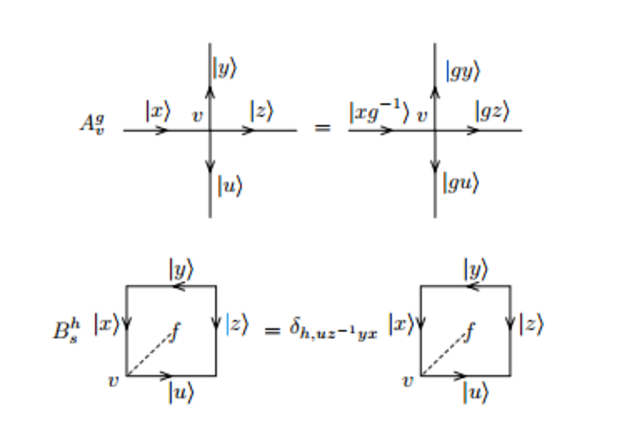
\includegraphics[width=10cm]{A_v_B_p.pdf}
\caption[Definition of Vertex, Face operators]{Definition of the $A_{v}^{g}$ and $B_{s}^{h}$ operators on a arbitrary vertex and face}
\centering
\label{fig:A_v_B_p operators}
\end{figure}

. The Hamiltonain for the lattice is given by 
\begin{center}
  $H = -\varSigma_{v} A_{v} - \varSigma_{f} B_{f}$
\end{center}

\subsection{Ribbon operators, Excitations, Anyon types}
    A ribbion $\xi$ in the lattice is a sequence of adjacent sites connecting two sites $s_{0}$ and $s_{1}$.
The ribbon operator $F^{h,g}_{\xi}$ is defined as in figure \ref{fig:ribbon} : \\
\begin{figure}
\centering
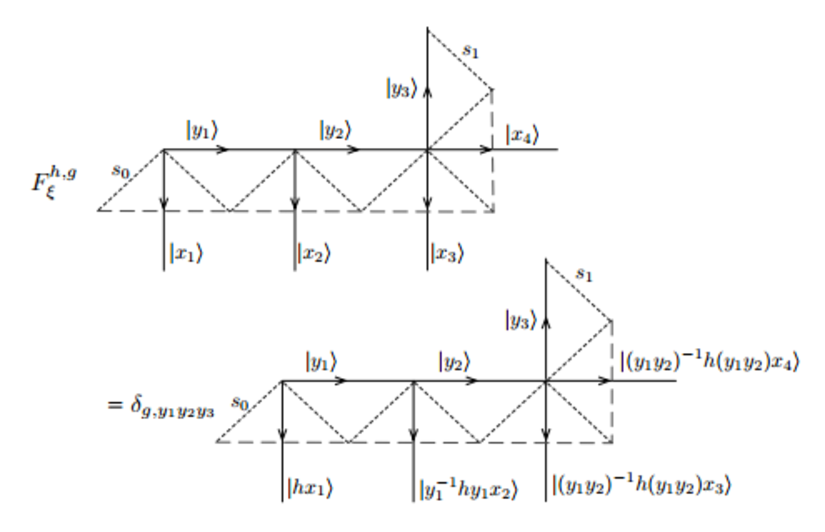
\includegraphics[width=10cm]{Ribbon_operator.pdf}
\caption[Definition of Ribbon operator]{Definition of a ribbon operator on a arbitrary lattice}
\centering
\label{fig:ribbon}
\end{figure}

For a ribbon connecting the sites $s_{0}$ and $s_{1}$, and if any site in the adjacent sequence is given by $t$,
the ribbon operator defined above satisfy the following commutation relationships,
\begin{center}
      [$F^{h,g}_{\xi}$, $A^{k}_{t}$] = [$F^{h,g}_{\xi}$, $B^{s}_{t}$] = 0, \\ 
      $A^{k}_{s_{0}}$ $F^{h,g}_{\xi}$ = $F^{khk^{-1},kg}_{\xi}$ $A^{k}_{s_{0}}$ \\
      $B^{k}_{s_{0}}$ $F^{h,g}_{\xi}$ = $F^{h,g}_{\xi}$ $B^{kh}_{s_{0}}$ \\
      $A^{k}_{s_{1}}$ $F^{h,g}_{\xi}$ = $F^{h,gk^{-1}}_{\xi}$ $A^{k}_{s_{1}}$ \\
      $B^{k}_{s_{1}}$ $F^{h,g}_{\xi}$ = $F^{h,g}_{\xi}$ $B^{g^{-1}h^{-1}gk}_{s_{1}}$
\end{center}

The application of ribbon operator on the ground state, gives rise to quasi-particle excitations at the end of the ribbon. The excitations are independent 
of the topology of the ribbon operator. Therefore the excitations can be moved around the lattice by extending/contracting the ribbon. Fusion of two quasi-particle
excitations can be achieved by moving them to the same site and fusing them, the resultant describes a system of anyons.

Anyon types for a Kitaev Quantum Double are in one-to-one correspondance with the irreducdible representations of the Drinfeld Double of the group, which are in 
one-to-one correspondace with the irreducible representations of the centralizers of the conjugacy classes of the group \citep{Reference1}. The method to compute this for any finite
group has been presented in Appendix \ref{AppendixA} and has been computed for various groups like $Z_{2}, S_{3}, D_{4}$ the first one being the case of Toric Code.

%----------------------------------------------------------------------------------------

\subsection{Introduction of boundaries, Condensates, Ribbon operators}

	Consider a lattice as above but with a boundary, that is with a lattice on one half and nothing on the other side, and the edges connecting both the half planes being
the boundary. The edges on the boundary are associated with a Hilbert space $C[K]$, where $C$ is the complex field and $K$ $\subset$ $G$ and indexed by elements of $K$. The 
vertex and the face operator for the internal lattice remain as defined in the introduction, but for the boundary the vertex and face operators are defined as follows :
\begin{center}
 $A^{K}_{s} = \frac{1}{|K|} \varSigma_{k \in K} A^{k}_{s}$ \\
 $B^{K}_{s} = \varSigma_{k \in K} B^{k}_{s}$
\end{center}
where $s$ is a site on the boundary.

The hamiltonian of the system with the boundary is given by,
\begin{center}
 $H = -\varSigma_{v} A_{v} - \varSigma_{f} B_{f} - \varSigma_{s} (A^{K}_{s} + B^{K}_{s})$
\end{center}

      To construct a ribbon $T = \varSigma_{h,g}c_{h,g}F^{h,g}_{\xi}$, connecting the sites in the bulk to the sites on the boundary, the ribbon should satisfy the commutation relationship mentioned in the 
previous section
\begin{center}
      $A^{k}_{s_{0}}$ $T$ = $T$ $A^{k}_{s_{0}}$ \\
      $B^{k}_{s_{0}}$ $T$ = $F^{h,g}_{\xi}$ $B^{kh}_{s_{0}}$ \\
\end{center}

along with the following commutation relationships :
\begin{center}
        $[T, A^{K}_{s_{0}}] = 0$ , \\
        $[T, B^{K}_{s_{0}}] = 0$
\end{center}

Solving for $T$, gives 
\begin{center}
    $T^{(k,g)} = \varSigma_{l \in K} F^{(lkl^{-1},lg^{-1})}_{\xi}$ 
\end{center}

We now present the various $T^{(k,g)}$ for the subgroups of $S_{3}$. Consider the subgroup 
$K$ = $G$, we compute the $T^{(k,g)}$ for various combinations of $k$ and $g$.

\subsubsection{Ribbon operators in a lattice with boundaries in the case of $S_{3}$}
Using the following snippet, we group the summation for each of the subgroup 
\begin{lstlisting}[frame=single]
sage: G =  SymmetricGroup(3)
sage: K = G.subgroups()[5]
sage: x = []
sage: y = []
sage: for k in K:
    for g in G:
        for l in K:
            x.append([l*k*l^-1, l*g^-1])
....: 
sage: for i in range(len(x)/6):
    y.append(x[6*i:6*(i+1)])

sage: y
# The first element is given by lkl^-1 and second element by lg^-1, which allows
# us to read  of the T^{(k,g)} from the first element of every summation. 

# For the case k = e and g running over all group elements.

[[[(), ()], [(), (2,3)], [(), (1,2,3)], [(), (1,2)], 
[(), (1,3,2)], [(), (1,3)]],
[[(), (1,2)], [(), (1,2,3)], [(), (2,3)], [(), ()], 
[(), (1,3)], [(), (1,3,2)]],
[[(), (1,3,2)], [(), (1,3)], [(), ()], [(), (2,3)], 
[(), (1,2,3)], [(), (1,2)]],
[[(), (1,2,3)], [(), (1,2)], [(), (1,3,2)], [(), (1,3)], 
[(), ()], [(), (2,3)]],
[[(), (2,3)], [(), ()], [(), (1,3)], [(), (1,3,2)], 
[(), (1,2)], [(), (1,2,3)]],
[[(), (1,3)], [(), (1,3,2)], [(), (1,2)], [(), (1,2,3)], 
[(), (2,3)], [(), ()]],

# Therefore, T^{(e,e)} is given by the first sum and similarly others. 
# So for the element e, the operators collapse to a single operator given by 
# T^{(e,g)} = summation(F^{(e,g)}) over all g \in G. Implying all the six collapse to a single operator.

# For the case k = (2,3) and g running over all group elements.

[[(2,3), ()], [(2,3), (2,3)], [(1,2), (1,2,3)], [(1,3), (1,2)], 
[(1,3), (1,3,2)], [(1,2), (1,3)]],
[[(2,3), (1,2)], [(2,3), (1,2,3)], [(1,2), (2,3)], [(1,3), ()], 
[(1,3), (1,3)], [(1,2), (1,3,2)]],
[[(2,3), (1,3,2)], [(2,3), (1,3)], [(1,2), ()], [(1,3), (2,3)], 
[(1,3), (1,2,3)], [(1,2), (1,2)]],
[[(2,3), (1,2,3)], [(2,3), (1,2)], [(1,2), (1,3,2)], [(1,3), (1,3)], 
[(1,3), ()], [(1,2), (2,3)]],
[[(2,3), (2,3)], [(2,3), ()], [(1,2), (1,3)], [(1,3), (1,3,2)],
[(1,3), (1,2)], [(1,2), (1,2,3)]],
[[(2,3), (1,3)], [(2,3), (1,3,2)], [(1,2), (1,2)], [(1,3), (1,2,3)],
[(1,3), (2,3)], [(1,2), ()]],
  
# In this case, (Performing a right multiplication gives the same results !)
# T^{((2,3), e)} = T^{((2,3), (2,3))}, 
# T^{((2,3), (1,2))} = T^{((2,3), (1,3,2))} 
# T^{((2,3), (1,2,3))} = T^{((2,3), (1,3))} 

# Therefore 6 operators reduce to 3.

# For the case k = (1,2,3) and g running over all group elements.

[[(1,2,3), ()], [(1,3,2), (2,3)], [(1,2,3), (1,2,3)], [(1,3,2), (1,2)],
[(1,2,3), (1,3,2)], [(1,3,2), (1,3)]],
[[(1,2,3), (1,2)], [(1,3,2), (1,2,3)], [(1,2,3), (2,3)], [(1,3,2), ()],
[(1,2,3), (1,3)], [(1,3,2), (1,3,2)]],
[[(1,2,3), (1,3,2)], [(1,3,2), (1,3)], [(1,2,3), ()], [(1,3,2), (2,3)],
[(1,2,3), (1,2,3)], [(1,3,2), (1,2)]],
[[(1,2,3), (1,2,3)], [(1,3,2), (1,2)], [(1,2,3), (1,3,2)], [(1,3,2), (1,3)],
[(1,2,3), ()], [(1,3,2), (2,3)]],
[[(1,2,3), (2,3)], [(1,3,2), ()], [(1,2,3), (1,3)], [(1,3,2), (1,3,2)],
[(1,2,3), (1,2)], [(1,3,2), (1,2,3)]],
[[(1,2,3), (1,3)], [(1,3,2), (1,3,2)], [(1,2,3), (1,2)], [(1,3,2), (1,2,3)],
[(1,2,3), (2,3)], [(1,3,2), ()]],

# In this case, again using the same rule as above it is easy to see
# T^{((1,2,3), e)} = T^{((1,2,3), (1,2,3))} = T^{((1,2,3), (1,3,2))}
# T^{((1,2,3), (1,2))} = T^{((1,2,3), (1,3))} = T^{((1,2,3), (2,3))}
  
# Therefore 6 operators collapse to 2.  

# For the case k = (1,2) and g running over all group elements.

[[(1,2), ()], [(1,3), (2,3)], [(1,3), (1,2,3)], [(1,2), (1,2)],
[(2,3), (1,3,2)], [(2,3), (1,3)]],
[[(1,2), (1,2)], [(1,3), (1,2,3)], [(1,3), (2,3)], [(1,2), ()],
[(2,3), (1,3)], [(2,3), (1,3,2)]],
[[(1,2), (1,3,2)], [(1,3), (1,3)], [(1,3), ()], [(1,2), (2,3)],
[(2,3), (1,2,3)], [(2,3), (1,2)]],
[[(1,2), (1,2,3)], [(1,3), (1,2)], [(1,3), (1,3,2)], [(1,2), (1,3)],
[(2,3), ()], [(2,3), (2,3)]],
[[(1,2), (2,3)], [(1,3), ()], [(1,3), (1,3)], [(1,2), (1,3,2)],
[(2,3), (1,2)], [(2,3), (1,2,3)]],
[[(1,2), (1,3)], [(1,3), (1,3,2)], [(1,3), (1,2)], [(1,2), (1,2,3)],
[(2,3), (2,3)], [(2,3), ()]]

# In this case, again using the same rule as above it is easy to see
# T^{((1,2), e)} = T^{((1,2), (1,2))}, 
# T^{((1,2), (1,3))} = T^{((1,2), (1,3,2))} 
# T^{((1,2), (1,2,3))} = T^{((1,2), (2,3))} 

# But in this case we also have 
# T^{((1,2), e)} = T^{((2,3), (1,2,3))}
# T^{((1,2), (1,3))} = T^{((2,3), e)}
# T^{((1,2), (1,2,3))} = T^{((2,3), (1,3,2))

# So again in this case 6  operators reduce to 3 but these are  mapped to the previous maps.

# For the case k = (1,3,2) and g running over all group elements.

[[(1,3,2), ()], [(1,2,3), (2,3)], [(1,3,2), (1,2,3)], [(1,2,3), (1,2)],
[(1,3,2), (1,3,2)], [(1,2,3), (1,3)]],
[[(1,3,2), (1,2)], [(1,2,3), (1,2,3)], [(1,3,2), (2,3)], [(1,2,3), ()],
[(1,3,2), (1,3)], [(1,2,3), (1,3,2)]],
[[(1,3,2), (1,3,2)], [(1,2,3), (1,3)], [(1,3,2), ()], [(1,2,3), (2,3)],
[(1,3,2), (1,2,3)], [(1,2,3), (1,2)]],
[[(1,3,2), (1,2,3)], [(1,2,3), (1,2)], [(1,3,2), (1,3,2)], [(1,2,3), (1,3)],
[(1,3,2), ()], [(1,2,3), (2,3)]],
[[(1,3,2), (2,3)], [(1,2,3), ()], [(1,3,2), (1,3)], [(1,2,3), (1,3,2)],
[(1,3,2), (1,2)], [(1,2,3), (1,2,3)]],
[[(1,3,2), (1,3)], [(1,2,3), (1,3,2)], [(1,3,2), (1,2)], [(1,2,3), (1,2,3)],
[(1,3,2), (2,3)], [(1,2,3), ()]],

# In this case, again using the same rule as above it is easy to see
# T^{((1,3,2), e)} = T^{((1,3,2), (1,3,2))} = T^{((1,3,2), (1,2,3))}
# T^{((1,2,3), (1,2))} = T^{((1,2,3), (1,3))} = T^{((1,2,3), (2,3))}

# But in this case we also have 
# T^{((1,3,2), e)} = T^{((1,2,3), (1,2))}
# T^{((1,3,2), (1,2))} = T^{((1,2,3), e)}

# As expected we have a reduction from 6 to 2, but these are  again mapped.

# For the case k = (1,2) and g running over all group elements.
[[(1,3), ()], [(1,2), (2,3)], [(2,3), (1,2,3)], [(2,3), (1,2)],
[(1,2), (1,3,2)], [(1,3), (1,3)]],
[[(1,3), (1,2)], [(1,2), (1,2,3)], [(2,3), (2,3)], [(2,3), ()],
[(1,2), (1,3)], [(1,3), (1,3,2)]],
[[(1,3), (1,3,2)], [(1,2), (1,3)], [(2,3), ()], [(2,3), (2,3)],
[(1,2), (1,2,3)], [(1,3), (1,2)]],
[[(1,3), (1,2,3)], [(1,2), (1,2)], [(2,3), (1,3,2)], [(2,3), (1,3)],
[(1,2), ()], [(1,3), (2,3)]],
[[(1,3), (2,3)], [(1,2), ()], [(2,3), (1,3)], [(2,3), (1,3,2)],
[(1,2), (1,2)], [(1,3), (1,2,3)]],
[[(1,3), (1,3)], [(1,2), (1,3,2)], [(2,3), (1,2)], [(2,3), (1,2,3)],
[(1,2), (2,3)], [(1,3), ()]]]

# In this case, again using the same rule as above it is easy to see
# T^{((1,3), e)} = T^{((1,3), (1,3))}, 
# T^{((1,3), (1,2,3))} = T^{((1,3), (1,2))} 
# T^{((1,3), (1,3,2))} = T^{((1,3), (2,3))} 

# But in this case we also have 
# T^{((1,3), e)} = T^{((1,2), (2,3))}
# T^{((1,3), (1,2,3))} = T^{((1,2), (1,3,2)}
# T^{((1,3), (1,3,2))} = T^{((1,2), (1,2))

# So again in this case 6  operators reduce to 3 but these are  mapped to the previous maps.

\end{lstlisting}

So in the above case where $K$ = $G$ we have reduced 36 operators to 6 unique operators.

Carrying out a similar analysis for $K$ = $\{e\}$, we again end up with 6 operators as follows :

\begin{lstlisting}[frame=single]
sage: G = SymmetricGroup(3)
sage: K = G.subgroups()[0]
sage: K
Subgroup of (Symmetric group of order 3! as a permutation group) generated by [()]
sage: for k in K:
    for g in G:
        for l in K:
            print k,g,l*k*l^-1, l*g^-1
....: 
() () () ()
() (1,2) () (1,2)
() (1,2,3) () (1,3,2)
() (1,3,2) () (1,2,3)
() (2,3) () (2,3)
() (1,3) () (1,3)
\end{lstlisting}

Hence the unique 6 operators are given by $T^{(e,e)}$, $T^{(e,(1,2))}$, $T^{(e,(2,3))}$, $T^{(e,(1,3))}$, $T^{(e,(1,2,3))}$, $T^{(e,(1,3,2))}$ give
out $F^{(e,e)}$, $F^{(e,(1,2))}$, $F^{(e,(2,3))}$, $F^{(e,(1,3))}$, $F^{(e,(1,2,3))}$, $F^{(e,(1,3,2))}$ in terms of $F_{\xi}^{(h,g)}$ which is defined on the sites.

Carrying out a similar analysis for $K$ = $\{e, \tau\}$, we again end up with 6 operators as follows :

\begin{lstlisting}[frame=single]
sage: G = SymmetricGroup(3)
sage: K = G.subgroups()[1]
sage: K
Subgroup of (Symmetric group of order 3! as a permutation group) generated by [(2,3)]
sage: for k in K:
    for g in G:
        for l in K:
            print k,g,l*k*l^-1, l*g^-1
() () () ()
() () () (2,3)
() (1,2) () (1,2)
() (1,2) () (1,2,3)
() (1,2,3) () (1,3,2)
() (1,2,3) () (1,3)
() (1,3,2) () (1,2,3)
() (1,3,2) () (1,2)
() (2,3) () (2,3)
() (2,3) () ()
() (1,3) () (1,3)
() (1,3) () (1,3,2)
(2,3) () (2,3) ()
(2,3) () (2,3) (2,3)
(2,3) (1,2) (2,3) (1,2)
(2,3) (1,2) (2,3) (1,2,3)
(2,3) (1,2,3) (2,3) (1,3,2)
(2,3) (1,2,3) (2,3) (1,3)
(2,3) (1,3,2) (2,3) (1,2,3)
(2,3) (1,3,2) (2,3) (1,2)
(2,3) (2,3) (2,3) (2,3)
(2,3) (2,3) (2,3) ()
(2,3) (1,3) (2,3) (1,3)
(2,3) (1,3) (2,3) (1,3,2) 
\end{lstlisting}

It is easy to see that the 12 operators reduce to unique 6, \\
$T^{(e,e)}$ = $F^{(e,e)}$ + $F^{(e,(2,3))}$, \\
$T^{(e,(1,2))}$ = $F^{(e,(1,2))}$ + $F^{(e,(1,2,3))}$, \\ 
$T^{(e,(1,2,3))}$ = $F^{(e,1,3,2)}$ + $F^{(e,(1,3))}$, \\
$T^{((2,3),e)}$ = $F^{((2,3),e)}$ + $F^{((2,3),(2,3))}$,\\
$T^{((2,3),(1,2))}$ = $F^{((2,3),(1,2))}$ + $F^{((2,3),(1,2,3))}$,\\
$T^{((2,3),(1,2,3)}$ = $F^{((2,3),(1,3,2))}$ + $F^{((2,3),(1,3))}$,\\

\subsubsection{Explicit Ribbon operators with boundary $K = \{e, \tau\} \subset S_{3}$ in terms of basis}
The section aims to present the explicit form of the operators generated in the case of $K$ = $\{e, \tau\}$,
in terms of the basis of the algebra of the ribbon operators \citep{Reference2}. The $F$ operators are represented 
in terms of the basis $F^{RC}u(i,j)v(i',j')$, where $R$ is the irreducible representation of the 
center of the conjugacy class $C$, is given by:
\begin{center}
$F_{\xi}^{h,g}$ = $\Sigma_{R \in {N_{C}}_{irred}} \Sigma_{j,j'=1}^{n_{R}} \Gamma^{j,j'}_{R}(n_{(h,g)})F^{RC}u(i,j)v(i',j')$ 
\end{center}
where $h^{-1} \in C$, $n_{(h,g)}$ = $q_{i(h^{-1})}^{-1}gq_{i(g^{-1}h^{-1}g)}$  Here $\Gamma$ is the unitary matrix representation of the element $n_{(h,g)}$. We list the representation of $S_3$ as it 
is the center of the conjugacy class of $e$.

\begin{tabular}{| l | l | l | l |}
 \hline 
 Elements  & 1-dim & 1-dim & 2-dim \\
 $e$       &  [1] & [1] &  $\begin{bmatrix}
			    1 & 0 \\
			    0 & 1 \\
			    \end{bmatrix}$ \\
 $(1,2,3)$ &  [1] & [1] & $\begin{bmatrix}
			    -\frac{1}{2} & \frac{\sqrt{3}}{2} \\
			    -\frac{\sqrt{3}}{2} & -\frac{1}{2} \\
			    \end{bmatrix}$ \\
 $(1,3,2)$ &  [1] & [1] & $\begin{bmatrix}
			    -\frac{1}{2} & -\frac{\sqrt{3}}{2} \\
			     \frac{\sqrt{3}}{2} & -\frac{1}{2} \\
			    \end{bmatrix}$ \\
 $(1,2)$   &  [1] & [-1] & $\begin{bmatrix}
			    -1 & 0 \\
			     0 & 1  \\
			    \end{bmatrix}$ \\
 $(2,3)$   &  [1] & [-1] & $\begin{bmatrix}
			    \frac{1}{2} & \frac{\sqrt{3}}{2} \\
			    \frac{\sqrt{3}}{2} & -\frac{1}{2} \\
			    \end{bmatrix}$ \\
 $(1,3)$   &  [1] & [-1] &  $\begin{bmatrix}
			    \frac{1}{2} & -\frac{\sqrt{3}}{2} \\
			    -\frac{\sqrt{3}}{2} & -\frac{1}{2} \\
			    \end{bmatrix}$\\
 \hline
\end{tabular}

$F^{(e,e)}$, here $h^{-1}$ is in the conjugacy class of $e$ and its centralizer is $S_{3}$ itself. So we have three irreps $\pi_{1}, \pi_{2}, \pi_{3}$ whose degrees are 1,1,2. Therefore $F^{(e,e)}$ 
is given by :
\begin{center}
$\Gamma^{1,1}_{\pi_{1}}(n_{(e,e)})F^{\pi_{1}\bar{e}}u(i,1)v(i',1) + \Gamma^{1,1}_{\pi_{2}}(n_{(e,e)})F^{\pi_{2}\bar{e}}u(i,1)v(i',1) 
              + \Gamma^{1,1}_{\pi_{3}}(n_{(e,e)})F^{\pi_{3}\bar{e}}u(i,1)v(i',1) + \Gamma^{1,2}_{\pi_{3}}(n_{(e,e)})F^{\pi_{3}\bar{e}}u(i,1)v(i',2)
              + \Gamma^{2,1}_{\pi_{3}}(n_{(e,e)})F^{\pi_{3}\bar{e}}u(2,1)v(i',1) + \Gamma^{2,2}_{\pi_{3}}(n_{(e,e)})F^{\pi_{3}\bar{e}}u(i,2)v(i',2)$
\end{center}
which reduces to 
\begin{center}
$F^{(e,e)}$ = $F^{\pi_{1}\bar{e}}u(i,1)v(i',1) + F^{\pi_{2}\bar{e}}u(i,1)v(i',1) 
              + F^{\pi_{3}\bar{e}}u(i,1)v(i',1) + F^{\pi_{3}\bar{e}}u(i,2)v(i',2)$
\end{center}

$F^{(e,(2,3))}$ is given by a similar structure, noting that $n_{(e,(2,3))} = (2,3)$, therefore the sum reduces to
\begin{center}
$F^{(e,(2,3))}$ = $F^{\pi_{1}\bar{e}}u(i,1)v(i',1) - F^{\pi_{2}\bar{e}}u(i,1)v(i',1) 
              + \frac{1}{2}F^{\pi_{3}\bar{e}}u(i,1)v(i',1) + \frac{\sqrt{3}}{2}F^{\pi_{3}\bar{e}}u(i,1)v(i',2)
              + \frac{\sqrt{3}}{2}F^{\pi_{3}\bar{e}}u(i,2)v(i',1) - \frac{1}{2}F^{\pi_{3}\bar{e}}u(i,2)v(i',2)$
\end{center}

Therefore  $T^{(e,e)}$ = $F^{(e,e)}$ + $F^{(e,(2,3))}$, is given by \\
\begin{center}
$T^{(e,e)}$ = $2F^{\pi_{1}\bar{e}}u(i,1)v(i',1) + \frac{3}{2}F^{\pi_{3}\bar{e}}u(i,1)v(i',1) 
                    + \frac{\sqrt{3}}{2}F^{\pi_{3}\bar{e}}u(i,1)v(i',2) + \frac{\sqrt{3}}{2}F^{\pi_{3}\bar{e}}u(i,2)v(i',1) 
                    + \frac{1}{2}F^{\pi_{3}\bar{e}}u(i,2)v(i',2)$
\end{center}

On similar lines, $T^{(e,(1,2))}$ = $F^{(e,(1,2))}$ + $F^{(e,(1,2,3))}$ we need to compute $F^{(e,(1,2))}$ and $F^{(e,(1,2,3))}$

For $F^{(e,(1,2))}$, we need $n_{(e,(1,2))} = (1,2)$ and hence 
\begin{center}
$F^{(e,(1,2))}$ = $F^{\pi_{1}\bar{e}}u(i,1)v(i',1) - F^{\pi_{2}\bar{e}}u(i,1)v(i',1) 
              - F^{\pi_{3}\bar{e}}u(i,1)v(i',1) + F^{\pi_{3}\bar{e}}u(i,2)v(i',2)$
\end{center}
For $F^{(e,(1,2,3))}$, we need $n_{(e,(1,2,3))} = (1,2,3)$ and hence
\begin{center}
$F^{(e,(1,2,3))}$ = $F^{\pi_{1}\bar{e}}u(i,1)v(i',1) + F^{\pi_{2}\bar{e}}u(i,1)v(i',1) 
              - \frac{1}{2}F^{\pi_{3}\bar{e}}u(i,1)v(i',1) + \frac{\sqrt{3}}{2}F^{\pi_{3}\bar{e}}u(i,1)v(i',2)
              - \frac{\sqrt{3}}{2}F^{\pi_{3}\bar{e}}u(i,2)v(i',1) - \frac{1}{2}F^{\pi_{3}\bar{e}}u(i,2)v(i',2)$
\end{center}

Therefore $T^{(e,(1,2))}$ is given by 
\begin{center}
$T^{(e,(1,2))}$ = $2F^{\pi_{1}\bar{e}}u(i,1)v(i',1) - \frac{3}{2}F^{\pi_{3}\bar{e}}u(i,1)v(i',1) 
                    + \frac{\sqrt{3}}{2}F^{\pi_{3}\bar{e}}u(i,1)v(i',2) - \frac{\sqrt{3}}{2}F^{\pi_{3}\bar{e}}u(i,2)v(i',1) 
                    + \frac{1}{2}F^{\pi_{3}\bar{e}}u(i,2)v(i',2)$
\end{center}

On similar lines, $T^{(e,(1,2,3))}$ = $F^{(e,(1,3,2))}$ + $F^{(e,(1,3))}$ we need to compute $F^{(e,(1,3,2))}$ and $F^{(e,(1,3))}$

For $F^{(e,(1,3,2))}$, we need $n_{(e,(1,3,2))} = (1,3,2)$ and hence 
\begin{center}
$F^{(e,(1,3,2))}$ = $F^{\pi_{1}\bar{e}}u(i,1)v(i',1) + F^{\pi_{2}\bar{e}}u(i,1)v(i',1) 
              - \frac{1}{2}F^{\pi_{3}\bar{e}}u(i,1)v(i',1) - \frac{\sqrt{3}}{2}F^{\pi_{3}\bar{e}}u(i,1)v(i',2)
              + \frac{\sqrt{3}}{2}F^{\pi_{3}\bar{e}}u(i,2)v(i',1) - \frac{1}{2}F^{\pi_{3}\bar{e}}u(i,2)v(i',2)$
\end{center}
For $F^{(e,(1,3))}$, we need $n_{(e,(1,3))} = (1,3)$ and hence
\begin{center}
$F^{(e,(1,3))}$ = $F^{\pi_{1}\bar{e}}u(i,1)v(i',1) - F^{\pi_{2}\bar{e}}u(i,1)v(i',1) 
              + \frac{1}{2}F^{\pi_{3}\bar{e}}u(i,1)v(i',1) - \frac{\sqrt{3}}{2}F^{\pi_{3}\bar{e}}u(i,1)v(i',2)
              - \frac{\sqrt{3}}{2}F^{\pi_{3}\bar{e}}u(i,2)v(i',1) - \frac{1}{2}F^{\pi_{3}\bar{e}}u(i,2)v(i',2)$
\end{center}

Therefore $T^{(e,(1,3,2))}$ is given by 
\begin{center}
$T^{(e,(1,3,2))}$ = $2F^{\pi_{1}\bar{e}}u(i,1)v(i',1) - \sqrt{3}F^{\pi_{3}\bar{e}}u(i,1)v(i',2) 
                    -F^{\pi_{3}\bar{e}}u(i,2)v(i',2)$
\end{center}


% $T^{((2,3),e)}$ = $F^{((2,3),e)}$ + $F^{((2,3),(2,3))}$,\\
% $T^{((2,3),(1,2))}$ = $F^{((2,3),(1,2))}$ + $F^{((2,3),(1,2,3))}$,\\
% $T^{((2,3),(1,2,3)}$ = $F^{((2,3),(1,3,2))}$ + $F^{((2,3),(1,3))}$,\\

On similar lines, $T^{((2,3),e)}$ = $F^{((2,3),e)}$ + $F^{((2,3),(2,3))}$ we need to compute $F^{((2,3),e)}$ and $F^{((2,3),(2,3))}$

For $F^{((2,3),e)}$, we need $n_{((2,3),e)} = e$ and hence 
\begin{center}
$F^{((2,3),e)}$ = $F^{\pi_{1}\bar{\tau}}u(i,1)v(i',1) + F^{\pi_{2}\bar{\tau}}u(i,1)v(i',1)$
\end{center}

For $F^{((2,3),(2,3))}$, we need $n_{((2,3),(2,3))} = (2,3)$ and hence
\begin{center}
$F^{(2,3),e}$ = $F^{\pi_{1}\bar{\tau}}u(i,1)v(i',1) - F^{\pi_{2}\bar{\tau}}u(i,1)v(i',1)$
\end{center}

Therefore $T^{(2,3),e)}$ is given by 
\begin{center}
$T^{((2,3),e)}$ = $2F^{\pi_{1}\bar{\tau}}u(i,1)v(i',1)$ % v lo i' index vary avutundi adi calculation chubettali
\end{center}

Similarly we have the other two ribbon operators given by 

\begin{center}
$T^{((2,3),(1,2))}$ = $2F^{\pi_{1}\bar{\tau}}u(i,1)v(i',1)$ % v lo i' index vary avutundi adi calculation chubettali
\end{center}

\begin{center}
$T^{((2,3),(1,2,3))}$ = $2F^{\pi_{1}\bar{\tau}}u(i,1)v(i',1)$ % v lo i' index vary avutundi adi calculation chubettali
\end{center}

Here the $i'$ varies over 1,2,3, giving rise to different $T$ operators. 

The above representation was computed with an idea to further reduce the number of operators, with an expectation of compressing 6 operators 
to three which further give rise to three ground states (thus verifying the fact that there are three ground states in the given system). 
But, as seen this happens to be a basis transformation, the calculation of the ground state is presented in the next section.

\subsubsection{Excitation condensation on various boundaries for $D(S_{3})$}
           The excitations in a Quantum Double model are given by irreps of the centralizers of the conjugacy class of the group. The character of a particular
representation $\pi$ is given by  $\chi_{(\bar{a}, \pi)}$ : 
\begin{center}
$\chi_{(\bar{a}, \pi)}(gh^{*}) = \delta_{h\in\bar{a}}\delta_{gh, hg} tr_{\pi}(k_{h}^{-1}gk_{h})$, 
\end{center}
as $h\in\bar{a}$ is one of the conditions to be satisfied, $k_{h}$ is some element in $G$ such that $h = k_{h}ak_{h}^{-1}$

For $k \in K$ and $g \in G$ define $|\psi^{k,g}_{K}> = T^{(k,g)} |\psi_{K}>$ and let $A(K)$ be the span of these vectors. Let $\chi_{A(K)}$ be the 
character of the representation $A(K)$. 
\begin{center}
$\chi_{A(K)}(hg^{*}) = \frac{1}{|K|}\delta_{gh,hg}\varSigma_{x \in G}\delta_{xgx^{-1} \in K}\delta_{xhx^{-1} \in K}$
\end{center}

To compute whether a particular excitation condenses at the boundary, the inner product defined as 
\begin{center}
 $<\chi_{1}, \chi_{2}> = \frac{1}{|G|} \varSigma_{g,h}(\chi_{1}(gh^{*})^{*}\chi_{2}(gh^{*})$
\end{center}
of the above characters is observed, if it is positive the excitation associated with the irrep of $D(G)$ condenses at the boundary.

Consider the case of $S_{3}$, the following are the conjugacy classes $\{e\}$, $\{\tau\}$ and $\{\sigma\}$ where $\{e, \tau, \sigma\}$ form the presentation of the group.
The corresponding centralizer for each of the conjugacy classes are given by $S_{3}$, $\{e, \tau\}$, $\{e, \sigma, \sigma^{-1}\}$, whose corresponding irreps are
$\{1$, sign, $\pi\}$, (where $1$, sign are one dimensional irreps of $S_{3}$ and $\pi$ is a two dimensional irrep.),  $\{1, -1\}$, $\{1, \omega, \omega^{*}\}$. For
the case of $S_{3}$ the irreps of $D(S_{3})$ are indexed by $V_{a, \pi}$ where $\pi$ is the representation of the centralizer of the conjugacy class of $a$.
Put together there are eight excitations in $D(S_{3})$ given by $V_{e, \pi_{1}}$, $V_{e, \pi_{2}}$, $V_{e, \pi_{3}}$, $V_{\tau, \pi_{1}}$, $V_{\tau, \pi_{2}}$, 
$V_{\sigma, \pi_{1}}$, $V_{\sigma, \pi_{2}}$, $V_{sigma, \pi_{3}}$ which are labelled and referred by $A, B, C, D, E, F, G, G$.
The following snippet has been used to compute the inner product, 
\begin{lstlisting}[frame=single]
sage: def character_1_irred(G, subgroup, g, h):
    sum = 0
    if h*g == g*h:
        for i in G:
            if i*g*i^-1 in subgroup and i*h*i^-1 in subgroup:
                sum = sum + 1
    return sum/len(subgroup)
....: 
sage: def character_2_irred(G, conjugacy_class, g, h):
    k_h = 0
    for i in G:
        if h*i == i*conjugacy_class.an_element():
            k_h = i
            break
    if g*h == h*g and k_h != 0:
        return  k_h^-1*g*k_h
    else:
        return 0
\end{lstlisting}

In the above snippet the first function returns the irreducible character of $A(K)$. The second function returns the element on which the trace is to be calculated by relating to
the representation of the centralizer of the conjugacy class. 

$S_{3}$ is taken as an example to explain further. First the subgroups and the conjugacy classes of $S_{3}$ are presented. 

\begin{lstlisting}[frame=single]
sage: G = SymmetricGroup(3)
sage: for i in G.subgroups():
....:     print i
....: 
Subgroup of (Symmetric group of order 3! as a permutation group) 
generated by [()]
Subgroup of (Symmetric group of order 3! as a permutation group) 
generated by [(2,3)]
Subgroup of (Symmetric group of order 3! as a permutation group) 
generated by [(1,2)]
Subgroup of (Symmetric group of order 3! as a permutation group) 
generated by [(1,3)]
Subgroup of (Symmetric group of order 3! as a permutation group) 
generated by [(1,2,3)]
Subgroup of (Symmetric group of order 3! as a permutation group) 
generated by [(2,3), (1,2,3)]

sage: for i in G.conjugacy_classes():
....:     print i
....: 
Conjugacy class of cycle type [1, 1, 1] in 
Symmetric group of order 3! as a permutation group
Conjugacy class of cycle type [2, 1] in 
Symmetric group of order 3! as a permutation group
Conjugacy class of cycle type [3] in 
Symmetric group of order 3! as a permutation group
\end{lstlisting}

    Consider the subgroup K = G, and for each of the conjugacy classes the element on which the trace is to be calculated is presented :

\begin{lstlisting}[frame=single]
sage: G.subgroups()[5]
Subgroup of (Symmetric group of order 3! as a permutation group) 
generated by [(2,3), (1,2,3)]

sage: G.conjugacy_classes()[0]
Conjugacy class of cycle type [1, 1, 1] in 
Symmetric group of order 3! as a permutation group

sage: for i in G:
    for j in G:
        print (character_1_irred(G, G.subgroups()[5], i, j), 
               character_2_irred(G, G.conjugacy_classes()[0], i, j))
....: 
(1, ())
(1, (1,2))
(1, (1,2,3))
(1, (1,3,2))
(1, (2,3))
(1, (1,3))

sage: for i in G:
    for j in G:
        print (character_1_irred(G, G.subgroups()[5], i, j), 
               character_2_irred(G, G.conjugacy_classes()[1], i, j))
....: 
(1, ())
(1, ())
(1, ())
(1, (1,2))
(1, (1,2))
(1, (1,2))

sage: for i in G:
    for j in G:
        print (character_1_irred(G, G.subgroups()[5], i, j), 
               character_2_irred(G, G.conjugacy_classes()[2], i, j))
....: 
(1, ())
(1, ())
(1, (1,2,3))
(1, (1,3,2))
(1, (1,3,2))
(1, (1,2,3))
\end{lstlisting}

The reading of the list is as follows : the first loop reads the following :  
\begin{center}
1*$tr_{\pi_{i}}(e)$ + 1*$tr_{\pi_{i}}(1,2)$ + 1*$tr_{\pi_{i}}(2,3)$ + 1*$tr_{\pi_{i}}(1,3)$ + 1*$tr_{\pi_{i}}(1,2,3)$ + 1*$tr_{\pi_{i}}(1,3,2)$
\end{center}

The character table of $S_{3}$ is given by, which gives the trace of the irreducible representations (here in this case the irreducible representation 
of the centralizer of the conjugacy class of $e$ is same as the irreducible representations of group $S_{3}$) :

\begin{lstlisting}[frame=single]
sage: G.character_table()
[ 1 -1  1] - $\pi_{2}$
[ 2  0 -1] - $\pi_{3}$
[ 1  1  1] - $\pi_{1}$
\end{lstlisting}

Let the respective representations be $\pi_{1}$, $\pi_{2}$, $\pi_{3}$.
From the character table for the conjugacy class of $e$ have $V_{e, \pi_{1}}$ to be a condensate as the inner product is greater than zero.
Considering the  case of $\pi_{2}$ the inner product goes to zero therefore $V_{e, \pi_{2}}$ does not condense at the boundary. Similarly the case of 
$V_{e, \pi_{3}}$.

Consider the conjugacy class of $\{\tau\}$, the centralizer of the conjugacy classes has irreducible representations as 1 and -1. Reading from the 
second loop we have the inner product as the following :
\begin{center}
3*$tr_{\pi_{i}}(e)$ + 3*$tr_{\pi_{i}}(1,2)$
\end{center}
which	 is greater than zero for 1 and zero for -1. Therefore $V_{\tau, \pi_{1}}$ forms a condensate while the other does not.

Similarly for the conjugacy class of $\{\sigma\}$, the centralizer of the conjugacy class has irreducible representations as 1, $\omega$, and $\omega^{*}$.
The inner product is given by :
\begin{center}
2*$tr_{\pi_{i}}(e)$ + 2*$tr_{\pi_{i}}(1,2,3)$ + 2*$tr_{\pi_{i}}(1,3,2)$
\end{center}
Therefore $V_{\sigma, \pi_{1}}$ condense while the other two do not.

Therefore to conclude, in the case of $K=G$, A,D,F condense at the boundary. 

Now consider the subgroup K=$\{e\}$, we perform a similar analysis :

\begin{lstlisting}[frame=single]
sage: for i in G:
....:     for j in G:
....:         print (character_1_irred(G, G.subgroups()[0], i, j), 
                     character_2_irred(G, G.conjugacy_classes()[0], i, j))
....: 
(6, ())
\end{lstlisting}

For the conjugacy class of $e$ we end up with the following  expression for the inner product :
\begin{center}
6*$tr_{\pi_{i}}(e)$,for each of $\pi_{i}$ 
\end{center}
the inner product is observed to be greater than zero. Therefore $V_{e, \pi_{i}}$, for $i$ = 1,2,3 condense at the 
boundary. 

Therefore to conclude, in the case of $K={e}$, A,B,C condense at the boundary. 

For the other two conjugacy classes i.e., $\{\tau\}$ and $\{\sigma\}$ the inner product goes to zero, therefore none of the excitations indexed by this space
condense at the boundary.

Consider the subgroup K=$\{e, \tau\}$, we have the following :

\begin{lstlisting}[frame=single]
sage: for i in G:
    for j in G:
        print (character_1_irred(G, G.subgroups()[1], i, j), 
               character_2_irred(G, G.conjugacy_classes()[0], i, j))
....: 
(3, ())
(1, (1,2))
(1, (2,3))
(1, (1,3))

sage: for i in G:
    for j in G:
        print (character_1_irred(G, G.subgroups()[1], i, j), 
               character_2_irred(G, G.conjugacy_classes()[1], i, j))
....: 
(1, ())
(1, ())
(1, ())
(1, (1,2))
(1, (1,2))
(1, (1,2))

sage: for i in G:
    for j in G:
        print (character_1_irred(G, G.subgroups()[1], i, j), 
               character_2_irred(G, G.conjugacy_classes()[2], i, j))
....: 
\end{lstlisting}

The above results imply the following :
For the conjugacy class of $e$, the inner product results in the following:
\begin{center}
3*$tr_{\pi_{i}}(e)$ + 1*$tr_{\pi_{i}}(1,2)$ + 1*$tr_{\pi_{i}}(2,3)$ + 1*$tr_{\pi_{i}}(1,3)$
\end{center}
which results in a value greater than zero for i=1 and i=3. Therefore $V_{e, \pi_{1}}$, $V_{e, \pi_{3}}$
condense at the boundary while $V_{e, \pi_{2}}$ do not.

Looking through the second loop gives the following :
\begin{center}
3*$tr_{\pi_{i}}(e)$ + 3*$tr_{\pi_{i}}(1,2)$ 
\end{center}
which results  in a  value greater than zero for the trivial representation that is $\pi_{1}$ while the other 
goes to zero.  Therefore $V_{\tau, \pi_{1}}$ condense at the boundary.

Therefore, A,C,D condense at the boundary.

Note : These results hold for all 2-cycle subgroups i.e., they belong to the same conjugacy class.


Finally we consider the subgroup K=$\{e, \sigma, \sigma^{-1}\}$ :

\begin{lstlisting}[frame=single]
sage: for i in G:
    for j in G:
        print (character_1_irred(G, G.subgroups()[4], i, j), 
               character_2_irred(G, G.conjugacy_classes()[0], i, j))
....: 
(2, ())
(2, (1,2,3))
(2, (1,3,2))

sage: for i in G:
    for j in G:
        print (character_1_irred(G, G.subgroups()[4], i, j), 
               character_2_irred(G, G.conjugacy_classes()[1], i, j))
....: 

sage: for i in G:
    for j in G:
        print (character_1_irred(G, G.subgroups()[4], i, j), 
               character_2_irred(G, G.conjugacy_classes()[2], i, j))
....: 
(2, ())
(2, ())
(2, (1,2,3))
(2, (1,3,2))
(2, (1,3,2))
(2, (1,2,3))
\end{lstlisting}

Analysis of the results is as follows :
For the conjugacy class of $e$ we have the following sum
\begin{center}
2*$tr_{\pi_{i}}(e)$ + 2*$tr_{\pi_{i}}(1,2,3)$ + 2*$tr_{\pi_{i}}(1,3,2)$ 
\end{center}
For the representations $\pi_{1}$ and $\pi_{2}$ we have the inner product to be greater than zero, therefore
$V_{e, \pi_{1}}$, $V_{e, \pi_{2}}$ condense at the boundary.

None from the conjugacy class $\{\tau\}$ condense at the boundary.

While in the case of the conjugacy class $\{\sigma\}$ the inner product is as the following :
\begin{center}
4*$tr_{\pi_{i}}(e)$ + 2*$tr_{\pi_{i}}(1,2,3)$ + 2*$tr_{\pi_{i}}(1,3,2)$
\end{center}
which is greater than zero only when i=1.
Therefore $V_{\sigma, \pi_{1}}$ condense at the boundary.

Therefore A,B,F condense at the boundary.

Therefore to summarize :\\
For the subgroup K=$G$, $A, D, F$ condense \\
For the subgroup K=$\{e\}$,  $A, B, C$ condense \\
For the subgroup K=$\{e, \tau\}$, $A, C, D$ condense \\
For the subgroup K=$\{e, \sigma, \sigma^{-1}\}$, $A, B, F$ condense \\

\textbf{Calculating the number of times a particular excitation condenses at the boundary} \\
To calculate the number of times a particular excitation condenses at the boundary the following relation is used \citep{Reference1}:
\begin{center}
$\chi_{A(K)}$ = $\varSigma_{(a, \pi)}$ $\alpha_{(a, \pi)}*\chi_{(a, \pi)}$
\end{center}

Consider the case of K=$G$, from the code table result above observe that
\begin{center}
$\chi_{A(G)}$ = $\alpha_{(e, \pi_{1})}*\chi_{(e, \pi_{1})}$ + $\alpha_{(\tau, \pi_{1})}*\chi_{(\tau, \pi_{1})}$ + $\alpha_{(\sigma, \pi_{1})}*\chi_{(\sigma, \pi_{1})}$
\end{center}
observing that for $g$=$h$=$e$, $\chi_{A(G)}(g,h) = 1$, and $\chi_{(e, \pi_{1})}(g, h)$ = 1, implies $\alpha_{(e, \pi_{1})}$ = 1 similarly 
$\alpha_{(\tau, \pi_{1})}$, $\alpha_{(\sigma, \pi_{1})}$.  This is easy to see as $e$ does not belong to the conjugacy class of $\{\tau\}$ or $\{\sigma\}$.
So, $A, D, F$ condense only once at the boundary.

Consider the case of K=$\{e\}$, from the table observe that
\begin{center}
$\chi_{A(G)}$ = $\alpha_{(e, \pi_{1})}*\chi_{(e, \pi_{1})}$ + $\alpha_{(e, \pi_{2})}*\chi_{(e, \pi_{2})}$ + $\alpha_{(e, \pi_{3})}*\chi_{(e, \pi_{3})}$
\end{center}
observing $\chi_{A(G)}(g,h)$ = 6, and $\chi_{(e, \pi_{1})}(g, h)$ = 1, $\chi_{(e, \pi_{2})}(g, h)$ = 1, $\chi_{(e, \pi_{3})}(g, h)$ = 2 implies 
\begin{center}
$\alpha_{(e, \pi_{1})}$ + $\alpha_{(e, \pi_{2})}$ + 2*$\alpha_{(e, \pi_{3})}$ = 6, implying
$\alpha_{(e, \pi_{1})}$ = 1, $\alpha_{(e, \pi_{2})}$ = 1, $\alpha_{(e, \pi_{3})}$ = 2
\end{center}
So, $A,B$ condense once while $C$ condeses twice at the boundary.

For the subgroups K=$\{e, \tau\}$, $A,C,D$ form the condensates and   
\begin{center}
$\alpha_{(e, \pi_{1})}$ = 1, $\alpha_{(e, \pi_{3})}$ = 1, $\alpha_{(\tau, \pi_{3})}$ = 1
\end{center}
So $A, C, D$ condense once at the boundary.

For the subgroups K=$\{e, \sigma, \sigma^{-1}\}$, $A, B, F$ form the condensates and from the table    
\begin{center}
$\alpha_{(e, \pi_{1})}$ = 1, $\alpha_{(e, \pi_{2})}$ = 1, $\alpha_{(\sigma, \pi_{1})}$ = 2
\end{center}
So $A, B$ condense once at the boundary, while $F$ condenses  twice at the boundary.


\subsection{Computing the ground state with respect to different $T$ operators on a single lattice cylinder:}
    
     Consider a single lattice i.e., identified by two vertices and a single edge. For this given construction, the ground state is computed by 
eigenstates of $A_{v}^{k}B_{p}^{e}T$ (equivalent to the action of $\Pi(\Sigma_{v}A_{v}^{k}) \Pi B_{p}$ on the eigenstates of opertor $T$). The general construction of state is given by 

\begin{center}
  
--$g_{1}$------$g_{1}$--\\
	   $|$\\
	   $|$\\
	 $g_{2}$\\
	   $|$\\
	   $|$	\\
--$g_{3}$------$g_{3}$--\\
\end{center}
where $g_{1}$, $g_{3}$ $\in$ $K$ subset of $G$. $g_{2}$ is a group element.


I. In the case of $T^{(e,e)}$ = $F^{(e,e)}$ + $F^{(e,(2,3))}$, the following form the eigenstates \\
For all  $g_{1}, g_{3}$ $\in$ $K$, $g_{2}$ is restricted to  $\{e, (2,3)\}$ (from the defintion of ribbon operator in 2.1).
So for each of $g_{2}$ the following condition must be satisfied (comes from the flux operator) $g_{3}g_{2}g_{1}g_{2}^{-1} =  e$.

So for $g_{2} =  e$, $g_{1}, g_{3}$ both are either going to  $(2,3)$ or both going to $e$. For each of the case the eigen state
(which is calculated by action of $A_{v}$ at different vertices one after the other and sum of all these terms). Let the upper vertex 
is acted by $k_{u}$ and the lower vertex by $k_{d}$ both of which come from the subgroup $K$. So there are four combinations for a given
($(k_{u}, k_{d}) = \{(e,e), (e, (2,3)), ((2,3),e), ((2,3), (2,3))\}$)  state which need to be added. The action on these vertices gives 
a variation of $g_{1}, g_{2}, g_{3}$ which get mapped to  $k_{u}g_{1}k_{u}^{-1}, k_{d}g_{2}k_{u}^{-1}, k_{d}g_{3}k_{d}^{-1}$. 
To evaluate this sum the following snippet has been used :

\begin{lstlisting}[frame=single]
sage: def ground_state(g1, g2, g3, ku, kd):
    return ku*g1*ku^-1, kd*g2*ku^-1, kd*g3*kd^-1

# for g_2 = e, g_1 = (2,3), g_3 = (2,3) 
sage: for i in G.subgroups()[1]:
    for j in G.subgroups()[1]:
        print ground_state(G[4], G[0], G[4], i, j)
....: 
((2,3), (), (2,3))
((2,3), (2,3), (2,3))
((2,3), (2,3), (2,3))
((2,3), (), (2,3))
\end{lstlisting}

So for $g_{2} = e, g_{1} = g_{3} = (2,3)$, the sum is the following : 
$\tau*e*\tau + \tau*\tau*\tau + \tau*\tau*\tau + \tau*e*\tau$

Similarly for the case $g_{2} = e, g_{1} = g_{3} = e$,
\begin{lstlisting}[frame=single]
sage: for i in G.subgroups()[1]:
    for j in G.subgroups()[1]:
        print ground_state(G[0], G[0], G[0], i, j)
....: 
((), (), ())
((), (2,3), ())
((), (2,3), ())
((), (), ())
\end{lstlisting}

So for $g_{2} = e, g_{1} = g_{3} = e$, the sum is 
$e*e*e + e*\tau*e + e*\tau*e + e*e*e$

Similarly for the case $g_{2} = (2,3), g_{1} = g_{3} = e$, 
\begin{lstlisting}[frame=single]
sage: for i in G.subgroups()[1]:
    for j in G.subgroups()[1]:
        print ground_state(G[0], G[4], G[0], i, j)
....: 
((), (2,3), ())
((), (), ())
((), (), ())
((), (2,3), ())
\end{lstlisting}

So for $g_{2} = (2,3), g_{1} = g_{3} = e$,
$e*\tau*e + e*e*e + e*e*e + e*\tau*e$

Similarly for the case $g_{2} = (2,3), g_{1} = g_{3} = (2,3)$, 
\begin{lstlisting}[frame=single]
sage: for i in G.subgroups()[1]:
    for j in G.subgroups()[1]:
        print ground_state(G[4], G[4], G[4], i, j)
....: 
((2,3), (2,3), (2,3))
((2,3), (), (2,3))
((2,3), (), (2,3))
((2,3), (2,3), (2,3))
\end{lstlisting}

So for $g_{2} = (2,3), g_{1} = g_{3} = e$, 
$\tau*\tau*\tau + \tau*e*\tau + \tau*e*\tau + \tau*\tau*\tau$

So in this case we have 2 ground states.

II. In the case of $T^{(e,(1,2))}$ = $F^{(e,(1,2))}$ + $F^{(e,(1,2,3))}$, the eigenstates look as follows : \\
For all  $g_{1}, g_{3}$ $\in$ K, $g_{2}$ is restricted to  $\{(1,2), (1,2,3)\}$ (the condition on $F$ operator).
So for each of $g_{2}$ the following condition must be satisfied (comes from the flux operator) $g_{3}g_{2}g_{1}g_{2}^{-1} =  e$.
 
So for $g_{2} = (1,2)$, $g_{1} = g_{3} = e$,  
\begin{lstlisting}[frame=single]
sage: for i in G.subgroups()[1]:
    for j in G.subgroups()[1]:
        print ground_state(G[0], G[1], G[0], i, j)
....: 
((), (1,2), ())
((), (1,2,3), ())
((), (1,3,2), ())
((), (1,3), ())
\end{lstlisting}

So for $g_{2} = (1,2), g_{1} = g_{3} = e$, 
$e*(1,2)*e + e*(1,2,3)*e + e*(1,3,2)*e + e*(1,3)*e$

Similarly for $g_{2} = (1,2,3)$, $g_{1} = g_{3} = e$, 
\begin{lstlisting}[frame=single]
sage: for i in G.subgroups()[1]:
    for j in G.subgroups()[1]:
        print ground_state(G[0], G[2], G[0], i, j)
....: 
((), (1,2,3), ())
((), (1,2), ())
((), (1,3), ())
((), (1,3,2), ())
\end{lstlisting}

Hence the sum is $e*(1,2)*e + e*(1,2,3)*e + e*(1,3,2)*e + e*(1,3)*e$

III. In the case of $T^{(e,(1,2,3))}$ = $F^{(e,(1,3))}$ + $F^{(e,(1,3,2))}$, following are the eigenstates \\
For all  $g_{1}, g_{3}$ $\in$ K, $g_{2}$ is restricted to  $\{(1,3), (1,3,2)\}$.
So for each of $g_{2}$ the following condition must be satisfied (comes from the flux operator) $g_{3}g_{2}g_{1}g_{2}^{-1} =  e$.

So for $g_{2} = (1,3)$, $g_{1} = g_{3} = e$,  
\begin{lstlisting}[frame=single]
sage: for i in G.subgroups()[1]:
    for j in G.subgroups()[1]:
        print ground_state(G[0], G[5], G[0], i, j)
....: 
((), (1,3), ())
((), (1,3,2), ())
((), (1,2,3), ())
((), (1,2), ())
\end{lstlisting}

So for $g_{2} = (1,3), g_{1} = g_{3} = e$, 
$e*(1,2)*e + e*(1,2,3)*e + e*(1,3,2)*e + e*(1,3)*e$

Similarly for $g_{2} = (1,3,2)$, $g_{1} = g_{3} = e$, 
\begin{lstlisting}[frame=single]
sage: for i in G.subgroups()[1]:
    for j in G.subgroups()[1]:
        print ground_state(G[0], G[3], G[0], i, j)
....: 
((), (1,3,2), ())
((), (1,3), ())
((), (1,2), ())
((), (1,2,3), ())
\end{lstlisting}

Hence the sum is $e*(1,2)*e + e*(1,2,3)*e + e*(1,3,2)*e + e*(1,3)*e$

Similarly for the other three operators, the same linear combination of states is observed, thus 
for the boundary case $K = \{e, \tau\}$ we have 3 unique ground states.

For the calculation of the number of excitations, condensates on the boundary, ribbon operators,
and ground states in a more general setting refer to Appendix \ref{AppendixA}.
 
% Chapter 3

\chapter{Category Theory and Lattice Models} % Main chapter title

\label{Chapter3} % For referencing the chapter elsewhere, use \ref{Chapter3} 

\lhead{Chapter 3. \emph{Category Theory and Lattice Models}} % This is for the header on each page - perhaps a shortened title

%----------------------------------------------------------------------------------------

\section{Levin-Wen Models}
    The aim of this section is to introduce the most general structure used to classify topological phases of matter. This uses the concepts presented in Chapter
\ref{Chapter1} and it will be shown that the contents presented in Chapter \ref{Chapter2} will form a subclass of these models in Chapter \ref{Chapter4}. The String Net Model
or Levin-Wen Model \citep{Reference3} is defined on trivalent graph embedded to a closed oriented surface. The rules of the model are as follows : \\

\begin{itemize}
\item[1] String types : They are finite number of string types, and the set of string types is isomorphic to positive integers.\\
\item[2] Branching rules : Only certain string types are allowed to form a  vertex.\\
\item[3] String orientation : Every string has a dual type, which is directed in the opposite direction.
\end{itemize}

The universal features of the string net model are given by fig \ref{fig:Levin_Wen_features} :
\begin{figure}
  \centering
      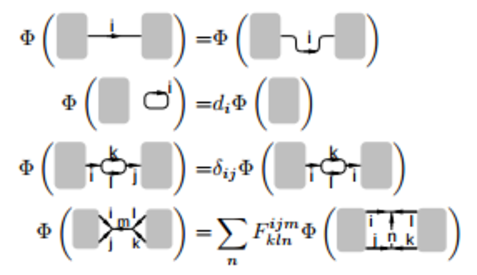
\includegraphics[width=8cm]{Levin_Wen_conditions.pdf}
      \caption[Features of Levin-Wen Model]{Universal features of the String-Net Model}
  \centering    
  \label{fig:Levin_Wen_features}
\end{figure}

Equivalently, they are captured by six index object $F_{ijk}^{klm}$ and the numbers $d_{i}$, that is the $F$ moves and the quantum dimensions. However not
all combinations of these give rise to string net model as they are constrainted by the above equations. The only valid combinations are those
which satisfy :
\begin{center}
$F^{ijk}_{j^{*}i^{*}0} = \frac{\sqrt{d_{k}}}{\sqrt{d_{i}d_{k}}}\delta_{ijk}$ \\
$F^{ijm}_{kln} = F^{klm^{*}}_{jin} = F^{jim}_{lkn^{*}} = F^{imj}_{k^{*}ln}\frac{\sqrt{d_{m}d_{n}}}{\sqrt{d_{j}d_{l}}}$ \\
$\varSigma_{n=0}^{N}F^{mlq}_{kp^{*}n}F^{jip}_{mns^{*}}F^{js^{*}n}_{lkr^{*}} = F^{jip}_{q^{*}kr^{*}}F^{riq^{*}}_{mls^{*}}$ 
\end{center}

Unitary Tensor Categories are the fundamental framework for the string net model. The string labels form the objects in category,
the Homspace can be seen as branching rules. Given a group $G$, the string labels are the irreducible representations of the group
$G$, the quantum dimension $d_{i}$ is the dimension of the representation, and the $F$ object is the $6j$ symbols of the group.

For every valid  $(F^{ijk}_{lmn}, d_{i})$,  the Hamiltonian of the model is given by :
\begin{center}
 $H = -\sum_{I}Q_{I} - \sum_{p}B_{p}$, where  $B_{p} = \sum_{s=0}^{N}a_{s}B_{p}^{s}$
\end{center}
where $Q_{I}$ measures the electric charge and favors no charge configuration, and $B_{p}$ measures the magnetic flux through a plaquette
and favors no flux. The figure \ref{fig:QvBp_Levin_Wen} give the action of $Q_{I}$ and $B_{\bold{p}}$ on a arbitrary lattice.
\begin{figure}
\centering

\includegraphics[width=9cm]{Q_I_LW.pdf}\\
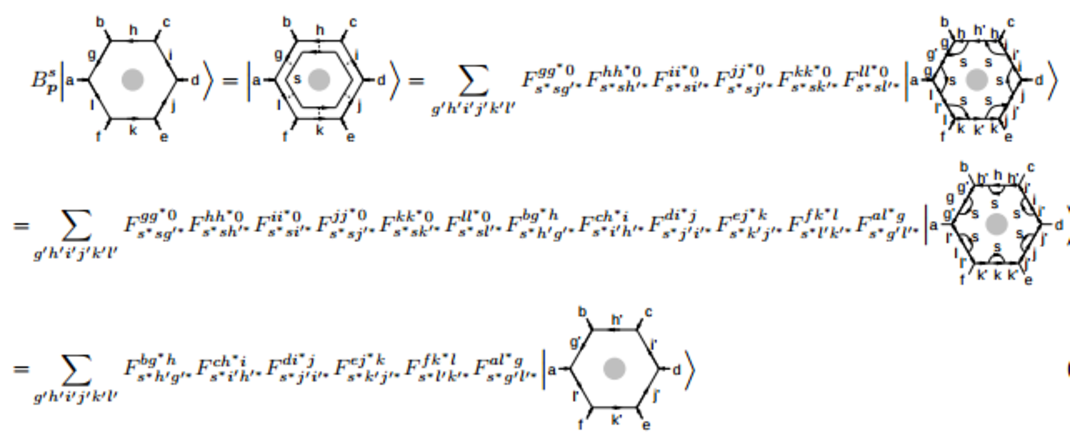
\includegraphics[width=15cm]{B_p_LW.pdf}
\caption[Vertex and Face operators in Levin-Wen model]{Definition of the $Q_{I}$ and $B_{p}$ operators}
\centering
\label{fig:QvBp_Levin_Wen}
\end{figure}
$Q_{I}$ and $B_{p}^{s}$ commute with each other, making the Hamiltonian exactly soluble. The ground state satisfies $Q_{I} = B_{p}^{s} = 1$ for
all $I, p$ while the excited states are those which violate these conditions. 

Given the strings are labelled by UTC $C$, the excitations are given by the monoidal center $Z(C)$ of the UTC $C$, which is a Modular Tensor Category. For example,
consider the Toric code $Z_{2}$, the strings are indexed by one dimensional representations, say, $1$ and $-1$ and the monoidal center of is given by the pair
$(M, \rho)$ where $\rho$ is given by $\rho : \_ \otimes M \rightarrow M \otimes \_ $, which in this case results in a category with rank four, these four form
the excitations in the Toric Code.

\section{Boundary construction, Condensations in String-Net model}

The following work by Kitaev and Kong \citep{Reference4}, presents the relationship between the UTC $C$ and the boundary labels. Consider a lattice with boundary, with edges being labelled
by $M$, which should satisfy all conditions mentioned in the previous section for a valid string-net configuration, that is they should be compatible with the $F$ moves.
Such a structure of the boundary is provided by the left module category over the UTC $C$. Therefore the edge labels on the boundary $M$ are given by the objects of left module category
over the UTC $C$. Given the bulk labels and the boundary labels it is possible to provide the Hamiltonian of the lattice. Once the Hamiltonian is defined, it should be possible 
to compute the ground state, which is used to compute the topological entanglement entropy.

Given the bulk of the lattice is labelled by simple objects from UTC $C$, the excitations are given by the center $Z(C)$ of the UTC $C$, which is a Modular Tensor Category.  
Using the above construction of Modular Tensor Category, the construction of the excitations  on the boundary, the construction of the condensed phase category can be achieved,
as mentioned below. For the detailed proof, refer to \citep{Reference5} \\

Consider the following construction, the excitations of a particular lattice given by UMTC $C$, the boundary excitations by UTC $E$, the condensed phase by another UMTC $D$. 

For one step condesations the following results hold :\\
\begin{itemize}
\item[1] Vacuum of $D$ is given by condensable algebra $A$ in $C$. (condensable implies the algebra is connected, commutative and separable) 
\item[2] $D \simeq C_{A}^{loc}$ category of local right $A$-modules in $C$. 
\item[3] $E \simeq C_{A}$ category of right $A$-modules in $C$. 
\item[4] Anyons in the bulk move onto the wall by the following functor map : 
\begin{center}
  $ \_ \otimes A : C \rightarrow  C_{A}$
\end{center}
\end{itemize}

For two step condensations the following results hold : \\
\begin{itemize}
\item[1] Vacuum in $D$ is given by condensable algebra $A$ in $C$. 
\item[2] $D$ is given by local right A-modules 
\item[3] Vacuum in $E$ is given by connected separable algebra $B$ in $C$. 
\item[4] $E$ is given by $B$-bimodule 
\item[5] Bulk to wall map from the $C$ side is given by :
\begin{center}
  $ \_ \otimes B : C \rightarrow : C_{B|B}$
\end{center}
\end{itemize}

The above statements provide an abstract insight into the relationship between the excitations in the bulk, on the boundary and the condensed phase. Though given the Modular Tensor Category, 
it is not totally possible to construct a lattice model with boundary, as there is no information of the labels in the bulk (the same MTC can be viewed as a center
of different UTC which are equivalent upto Morita equivalence) and also the labels on the boundary. 


% So given $C$, $D$, $E$ how do we find the algebras ! 
% (Indeed this is the one which would give us the boundary objects as well since in both one-step and two step condensations, 
% $E$ is given by right modules of the condensable algebra obtained identified as a vacuum for $D$ (but this reasoning is flawed 
% because we already are given $E$, so there is no need to find $E$. The question is this, given objects in $C'$ whose center 
% $Z(C') = C$, the algebras in $C$ will give us the objects on the boundary $E$ (right modules of the condesable algebras in $C$) 
% So it all boils down to answering the following question, how do we find the algebras in the MTC $C$ ?! \\

% $E$ is given by the Langangrian algebras in $C$.  \\

% For the Double Ising model, $C'$ is given by $1, \sigma, \psi$ and the boundary $E$ is also given by $1, \sigma, \psi$. \\

% The ground state is both the eigen-states of the operators $Q_{v}$ and $B_{p}$, where $Q_{v}$ are fusion rules and $B_{p}$ is given
% by $\varSigma (d_{k}/D^{2}) B_{p}^{k}$, we present the ground states but we do not know how to include excitations (ribbon operators) 
% in these kind of models.

% Construction of ground states on a cylinder with Ising x Ising : \\

% The following satisfy the $Q_{v}$ operator \\
% \begin{center}
% --$v_{1}$------$v_{1}$--\\
%	   $|$\\
%	   $|$\\
%	 $v_{2}$\\
%	   $|$\\
%	   $|$	\\
%--$v_{3}$------$v_{3}$--\\
%\end{center}
%$ (v1, v2, v3) = \{\{1,1,1\} - (1),\{\psi,1,\psi\} - (2),\{\psi,1,1\} - (3),\{\sigma,1,\psi\} - (4), \{\sigma,1,\sigma\} - (5), 
%                   \{\sigma,1,1\} - (6),\{\sigma,\psi,\sigma\} - (7), \{\psi,1,\sigma\} - (8),\{1,1,\sigma\} - (9),\{1,1,\psi\}\ - (10)\}$ \\

%The action of $B_{p}^{1}$ on the above set results in the same set. \\
%The action of $B_{p}^{\psi}$ on the above set results in the following $\{2,1,10,6,5,4,7,9,8,3\}$.\\
%The action of $B_{p}^{\sigma}$ on the above set results in the following 1/sqrt(2) times $\{5+7,5+7,5-7,8+9,1+2+3+10,8+9,1+2-3-10,4+6,4+6,3-7\}$.\\

% Hence we have the following matrices given by $B_p_1, B_p_psi, B_p_sigma$ : \\
%\begin{lstlisting}[frame=single]
%julia> B_p_1 = eye(10);                                                                                                                                                                                                       
%                                                                                                                                                                                                                              
%julia> B_p_psi = [[0 1 0 0 0 0 0 0 0 0]; [1 0 0 0 0 0 0 0 0 0]; [0 0 0 0 0 0 0 0 0 1]; 
%		  [0 0 0 0 0 1 0 0 0 0]; [0 0 0 0 1 0 0 0 0 0]; [0 0 0 1 0 0 0 0 0 0]; 
%		  [0 0 0 0 0 0 1 0 0 0]; [0 0 0 0 0 0 0 0 1 0]; [0 0 0 0 0 0 0 1 0 0]; 
%		  [0 0 1 0 0 0 0 0 0 0]];                                                                                                                                                                                                     
%                                                                                                                                                                                                                              
% julia> B_p_s = [[0 0 0 0 1 0 1 0 0 0]; [0 0 0 0 1 0 1 0 0 0]; [0 0 0 0 1 0 -1 0 0 0]; 
%		[0 0 0 0 0 0 0 1 1 0]; [1 1 1 0 0 0 0 0 0 1]; [0 0 0 0 0 0 0 1 1 0]; 
%		[1 1 -1 0 0 0 0 0 0 -1]; [0 0 0 1 0 1 0 0 0 0]; [0 0 0 1 0 1 0 0 0 0]; 
%		[0 0 0 0 1 0 -1 0 0 0]]                                                                                                                                                                                                   
%
%julia> B_p_sigma = 1/sqrt(2)*B_p_s;                                                                                                                                                                                          
%                                                                                                                                                                                                                              
%julia> B = (1/4)*(B_p_1 + B_p_psi + sqrt(2)*B_p_sigma);                                                                                                                                                                       
%                                                                                                                                                                                                                              
%julia> eigvals(inv(eigvecs(B))*B*eigvecs(B))                                                                                                                                                                                  
%10-element Array{Complex{Float64},1}:                                                                                                                                                                                         
%         -7.91813e-18+0.0im                                                                                                                                                                                                   
%                  1.0+0.0im                                                                                                                                                                                                   
% 8.82083e-18+8.37086e-18im                                                                                                                                                                                                    
% 8.82083e-18-8.37086e-18im                                                                                                                                                                                                    
%                  1.0+0.0im                                                                                                                                                                                                   
%                  1.0+0.0im                                                                                                                                                                                                   
%         -7.14582e-18+0.0im
% 1.27443e-18+1.57887e-18im 
% 1.27443e-18-1.57887e-18im 
%          1.42363e-18+0.0im
 
% julia> eigvecs(inv(eigvecs(B))*B*eigvecs(B))                                                                                                                                                                                  
% 10x10 Array{Complex{Float64},2}:

% \end{lstlisting}

% So for the case of $S_{3}$, the irreps of $D(S_{3})$ form the objects of MTC, while $Rep(S_{3})$ form the objects in UTC. So we need 
% to get the algebras of irreps of $D(S_{3})$ to get the boundaries and once we have the boundaries, we can get the ground state, but then 
% again we need the notion of ribbon operators, which is  missing and Yuting's paper must provide an insight !

\section{Excitations, String operators in String-Net Model}

The excitations in the model are those eigenvectors which do not satisfy the ground state conditions, if $Q_{v} = 0$ is violated the excitation
is a charge excitation at vertex $v$ and is identified by a non-trivial edge label attached to the vertex and if $B_{p}^{s}=0$ is violated 
a fluxon excitation is identified at the plaquette $p$. If all the tail labels are trivial, Levin-Wen lattice is recovered. The lattice with charges are 
invariant under the operators as defined in figure \ref{fig:T1_T4} :
\begin{figure}
\centering
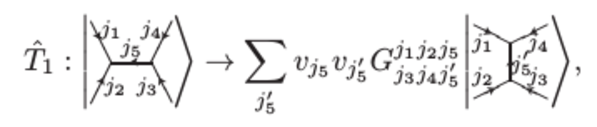
\includegraphics[width=8cm]{T_1_Dyon.pdf}\\
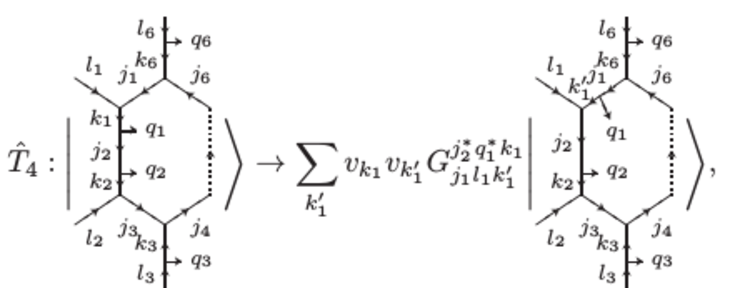
\includegraphics[width=8cm]{T_4_Dyon.pdf}
\caption[Invariant operators in Dyonic model]{Invariant operators in generalized Levin-Wen Model}
\centering
\label{fig:T1_T4}
\end{figure}
The first one is the $F$ move and the second is used to move the non-trivial label around the particular vertex.

The string operator $W_{e}^{J;pq^{*}}$ acting on a state, giving rise to the $J$ fluxon and charges $p$ and $q^{*}$, is as 
given in figure \ref{fig:String_operator}
\begin{figure}
\centering
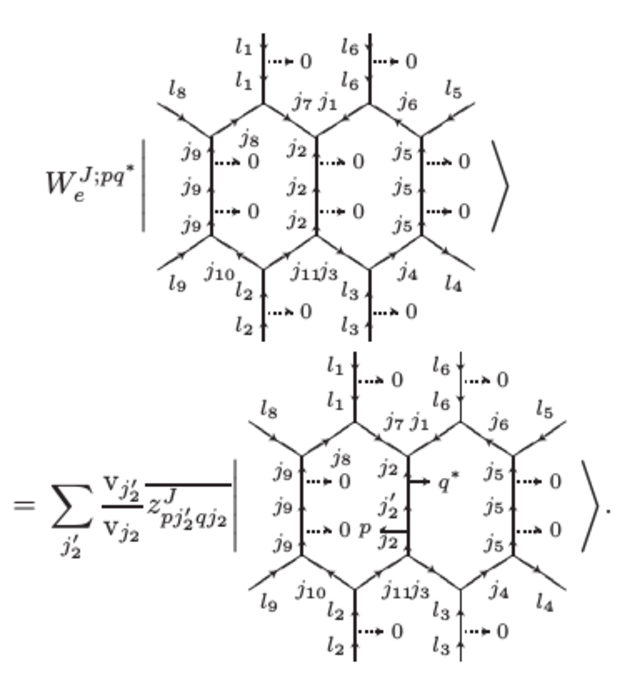
\includegraphics[width=8cm]{String_operator_dyon.pdf}
\caption[String operator in the Dyonic Model]{String operator in generalized Levin-Wen Model}
\centering
\label{fig:String_operator}
\end{figure}

String operator is the ribbon operator equivalent in the String-Net model. For various other operations on the string operators, the charge measurement,
the flux measurement and the action of $Q_{v}^{q}$ and $B_{p}^{s}$ refer to \citep{Reference6}.
% Chapter 3

\chapter{Quantum Doubles and other examples in String-Net picture} % Main chapter title

\label{Chapter4} % For referencing the chapter elsewhere, use \ref{Chapter3} 

\lhead{Chapter 4. \emph{Quantum Doubles and other examples in String-Net picture }} % This is for the header on each page - perhaps a shortened title

%----------------------------------------------------------------------------------------

\section{Toric Code, Quantum Double of $S_{3}$ in terms of Categories}
            As mentioned in the previous Chapter \ref{Chapter3}, the edge labelling is done by irreducible representations of the group, which forms a Unitary Tensor Category. 
The excitations are given by the monoidal center of the Unitary Tensor Category which is a Modular Tensor Category. This section aims to present some examples to realize the
above statements in case of Toric Code, $D(Z_{2})$ and $D(S_{3})$. 

\underline{$D(Z_{2})$, Toric Code}:\\
         The input to the Toric Code is the group $Z_{2}$, that is the edges are indexed by ${-1, 1}$. $Z_{2}$ has two one dimensional irreducible representations. These form
the data for the Unitary Tensor Category. The excitations are given by the center of the unitary tensor category. The objects in the center of the category $C$ are given by a pair 
$(M, \rho_{X})$ where $\rho_{X} : X \otimes M \rightarrow M \otimes X$, where $M, X$ $\in$ $C$. The irreducible representations of $Z_{2}$, say $V_{1}$ and $V_{-1}$ each branching 
into $(V_{1},\rho_{1})$, $(V_{1},\rho_{-1})$, $(V_{-1},\rho_{1})$, $(V_{-1},\rho_{-1})$. Therefore the rank of the modular tensor category is four and thus there are four excitations.

\underline{$D(S_{3})$} : \\
	The input to Quantum Double of $S_{3}$ is the group $S_{3}$. $S_{3}$ has two one dimensional and one two dimensional irreducible representations. These form the data for the Unitary Tensor Catgory. 
The excitations are given by the center of the representation category of $S_{3}$, which is isomorphic to the irreducible representations of the Drinfeld Double, which is indexed by irreducible 
representations of the centralizer of the conjugacy classes of the group. In this example, there are eight such objects. Each of the irreducible representation is a simple object in the Modular Tensor 
Category.
 
\section{Boundary construction for Toric Code, $D(S_{3})$}
      The boundary labels are given by objects of the left modules over $C$, $C_{M}$, where $C$ is a Unitary Tensor Category used to index the bulk. Consider the case of Kitaev Quantum 
Double $D(S_{3})$, the boundary labels were given by the subgroup $K \subset S_{3}$, from the definition of left module over a Unitary Tensor Category, it is easy to that the subgroups form the left modules. 
Thereby, the boundaries are indexed by various elements of the subgroups. 

      Consider the following construction, the excitations given by MTC $C$, the boundary excitations by $E$, the condensed phase by $D$. The boundary excitations are given by right $A$-modules in $C$, 
where $C$ is the Modular Tensor Category whose objects are the excitations of the lattice model. The vacuum in $D$ is a condensable algebra $A$ in $C$. For the toric code, suppose the excitations are labelled by 
$1, e, m, f$. $1 \oplus e$ and $1 \oplus m$ both are objects in $C$ and are algebras in $C$. This is easy to see from the graphical calculus viewpoint and also verifying the commutation relationships.
These in addition of being algebras, also satisfy the connected, commutative, separable properties making them condensable algebras. Hence these form the vacuum in the condensed phase. The detection of these
algebras sets the construction of not only $E$ and $D$, but also the excitations which condense on the boundary. Referring to the functor, the excitation to the wall map, in the case of Toric Code for the condensable
algebra $1 \oplus e$, the excitations $1, e$ are identified with $1 \oplus e$ and $f, m$ are identified with $ m \oplus e$.  $D$ itself is given by $1+e$, and $E$ is given by $m \oplus e$ and  $1 \oplus e$. 
The above construction provides an insight into the  excitations on the boundary, as well the excitations which condense on the boundary, but not the boundary labels. The above techniques can be extended to obtain the 
bulk excitations, the boundary excitations and the condensed phase for $D(S_{3})$ using the data from \citep{Reference7}.

\section{Ground state construction for lattice with Ising on boundary}
    Consider the following lattice model, the edges coming from the UTC of Ising whose objects are $1, \psi, \sigma$. The boundary labels also come from the UTC of Ising, as it forms a left-module of the bulk,
which is Ising. The ground state is both the eigen-states of the operators $Q_{v}$ and $B_{p}$, where $Q_{v}$ are fusion rules and $B_{p}$ is given by $\varSigma (d_{k}/D^{2}) B_{p}^{k}$. Consider a single lattice on the
cylinder. 
\begin{center}
--$v_{1}$------$v_{1}$--\\
	   $|$\\
	   $|$\\
	 $v_{2}$\\
	   $|$\\
	   $|$	\\
--$v_{3}$------$v_{3}$--\\
\end{center}
$ (v1, v2, v3) = \{\{1,1,1\} - (1),\{\psi,1,\psi\} - (2),\{\psi,1,1\} - (3),\{\sigma,1,\psi\} - (4), \{\sigma,1,\sigma\} - (5), 
                   \{\sigma,1,1\} - (6),\{\sigma,\psi,\sigma\} - (7), \{\psi,1,\sigma\} - (8),\{1,1,\sigma\} - (9),\{1,1,\psi\}\ - (10)\}$ \\

The action of $B_{p}^{1}$ on the above set results in the same set. \\
The action of $B_{p}^{\psi}$ on the above set results in the following $\{2,1,10,6,5,4,7,9,8,3\}$.\\
The action of $B_{p}^{\sigma}$ on the above set results in the following 1/sqrt(2) times $\{5+7,5+7,5-7,8+9,1+2+3+10,8+9,1+2-3-10,4+6,4+6,3-7\}$.\\

The matrices $B_{p}^{1}, B_{p}^{\psi}, B_{p}^{\sigma}$ are to used compute $B_{p}$ which is given by $\frac{1}{D}\sum_{s}d_{s}B_{p}^{s}$, which is further 
used to compute the ground states:  \\
\begin{lstlisting}[frame=single]
julia> B_p_1 = eye(10);                                                                                                                                                                                                       
                                                                                                                                                                                                                              
julia> B_p_psi = [[0 1 0 0 0 0 0 0 0 0]; [1 0 0 0 0 0 0 0 0 0]; [0 0 0 0 0 0 0 0 0 1]; 
		  [0 0 0 0 0 1 0 0 0 0]; [0 0 0 0 1 0 0 0 0 0]; [0 0 0 1 0 0 0 0 0 0]; 
		  [0 0 0 0 0 0 1 0 0 0]; [0 0 0 0 0 0 0 0 1 0]; [0 0 0 0 0 0 0 1 0 0]; 
		  [0 0 1 0 0 0 0 0 0 0]];                                                                                                                                                                                                     
                                                                                                                                                                                                                              
julia> B_p_s = [[0 0 0 0 1 0 1 0 0 0]; [0 0 0 0 1 0 1 0 0 0]; [0 0 0 0 1 0 -1 0 0 0]; 
		[0 0 0 0 0 0 0 1 1 0]; [1 1 1 0 0 0 0 0 0 1]; [0 0 0 0 0 0 0 1 1 0]; 
		[1 1 -1 0 0 0 0 0 0 -1]; [0 0 0 1 0 1 0 0 0 0]; [0 0 0 1 0 1 0 0 0 0]; 
		[0 0 0 0 1 0 -1 0 0 0]]                                                                                                                                                                                                   

julia> B_p_sigma = 1/sqrt(2)*B_p_s;                                                                                                                                                                                          
                                                                                                                                                                                                                              
julia> B = (1/4)*(B_p_1 + B_p_psi + sqrt(2)*B_p_sigma);                                                                                                                                                                       
                                                                                                                                                                                                                              
julia> eigvals(inv(eigvecs(B))*B*eigvecs(B))                                                                                                                                                                                  
10-element Array{Complex{Float64},1}:                                                                                                                                                                                         
         -7.91813e-18+0.0im                                                                                                                                                                                                   
                  1.0+0.0im                                                                                                                                                                                                   
8.82083e-18+8.37086e-18im                                                                                                                                                                                                    
8.82083e-18-8.37086e-18im                                                                                                                                                                                                    
                 1.0+0.0im                                                                                                                                                                                                   
                 1.0+0.0im                                                                                                                                                                                                   
        -7.14582e-18+0.0im
1.27443e-18+1.57887e-18im 
1.27443e-18-1.57887e-18im 
         1.42363e-18+0.0im
 
julia> eigvecs(inv(eigvecs(B))*B*eigvecs(B))                                                                                                                                                                                  
10x10 Array{Complex{Float64},2}:

% \end{lstlisting}
 
Thus, the number of ground states of the lattice with Ising both on bulk and boundary is three, which is in agreement with \citep{Reference8}.  
% Chapter 5

\chapter{Summary and Future Directions} % Main chapter title

\label{Chapter5} % For referencing the chapter elsewhere, use \ref{Chapter3} 

\lhead{Chapter 5. \emph{Summary and Future  Directions}} % This is for the header on each page - perhaps a shortened title

%----------------------------------------------------------------------------------------
\section{Summary}
      To summarize, we started with a brief introduction to category theory and some mathematical structures like Algebras, Bialgebras and Hopf Algebras which were used to construct the 
Drinfeld Double of a group. We then introduced the lattice models which are used to classify the topological phases of matter. Kitaev Quantum Double Models were introduced along with some
properties of the system like ground state construction, ribbon operator construction leading to detection of excitations given a particular group. Construction of ribbon operators in a Quantum 
Double with boundaries leading to detection of condensation of excitations on boundaries is presented. SageMath \citep{Reference9} has been used to compute the ribbon operators on lattice with boundaries, excitations
which condense on the boundary, the results for $S_{3}$ have been presented in thesis and for any generalized group the methods to compute the same have been presented in the Appendix \ref{AppendixA}. An introduction
to Levin-Wen models with and without boundaries, with a brief introduction to excitation detection and string operator that is the ribbon operator equivalent have been presented. Statements relating excitations in 
the bulk, excitations on the boundary and excitations in the condensed phase have been presented in one step as well as two step condensation. In the end, an attempt has been made to show Quantum Doubles
as a subclass of Levin-Wen models and various results have been verified in the case of the Toric Code and $D(S_{3})$.  
\pagebreak
\section{Future Directions}
      Some of the following ideas require further work :
\begin{itemize}
 \item Computing the commutation relationship equivalent of ribbon operators for string operators. Solving for string operators in the presence of boundary using the commutation relationship. For the 
       $Q_{v}$ operator, the result has been computed but $B_{p}$ operator is still a work in progress. Once the string operators in a lattice with boundaries are computed, the next step is to compute
       the ground state which would lead to the computation of topological entanglement entropy.
 \item Construction of ribbon operators in higher dimensions \citep{Reference10}.
 \item Construction of boundary conditions for Twisted Quantum Double models in 2D \citep{Reference11, Reference12} and 3D \citep{Reference13}, and extending the idea of ribbon operators for these models with boundaries.
 \item In the case of $D(S_{3})$, construction of condensable algebras play an important role as these would help in understanding the computation of boundary excitations, condensed phase and excitations which condense
       on the boundary.
 \item Topological Entanglement Entropy in the presence of ribbon operators in the case of $D(S_{3})$
 \item Given the center of a UTC which is a MTC, one can find many UTC's which are equivalent upto Morita equivalence. Given a UTC, one can construct the boundary labels as left modules of the UTC. Therefore, 
       given a MTC, is it possible to predict the boundary labels.
 \item Understanding of co-dimension 2 boundaries and application to the case of $D(S_{3})$.
 \item The ribbon operators computed for $S_{3}$ do not provide the required insight on splitting of excitation on boundary. In the sense the action of the ribbon operator on a cylinderical lattice 
       connecting boundaries at the top and bottom, is equivalent to the horizontal surface action. The construction of ribbon operator with vertical surface action might provide an insight into the 
       splitting of excitation on boundary.
 
\end{itemize}
 
%\input{Chapters/Chapter6} 
%% Chapter 1

\chapter{Reference} % Main chapter title

\label{Chapter3} % For referencing the chapter elsewhere, use \ref{Chapter1} 

\lhead{Chapter 3. \emph{TeX reference}} % This is for the header on each page - perhaps a shortened title

%----------------------------------------------------------------------------------------

\subsection{Common \LaTeX{} Math Symbols}
There are a multitude of mathematical symbols available for \LaTeX{} and it would take a great effort to learn the commands for them all. The most common ones you are likely to use are shown on this page:\\
\href{http://www.sunilpatel.co.uk/latexsymbols.html}{\texttt{http://www.sunilpatel.co.uk/latexsymbols.html}}

You can use this page as a reference or crib sheet, the symbols are rendered as large, high quality images so you can quickly find the \LaTeX{} command for the symbol you need.

\subsection{\LaTeX{} on a Mac}
 
The \LaTeX{} package is available for many systems including Windows, Linux and Mac OS X. The package for OS X is called MacTeX and it contains all the applications you need -- bundled together and pre-customised -- for a fully working \LaTeX{} environment and workflow.
 
MacTeX includes a dedicated \LaTeX{} IDE (Integrated Development Environment) called ``TeXShop'' for writing your `\texttt{.tex}' files and ``BibDesk'': a program to manage your references and create your bibliography section just as easily as managing songs and creating playlists in iTunes.

%----------------------------------------------------------------------------------------

\section{Getting Started with this Template}

If you are familiar with \LaTeX{}, then you can familiarise yourself with the contents of the Zip file and the directory structure and then place your own information into the `\texttt{Thesis.cls}' file. Section \ref{FillingFile} on page \pageref{FillingFile} tells you how to do this. Make sure you read section \ref{ThesisConventions} about thesis conventions to get the most out of this template and then get started with the `\texttt{Thesis.tex}' file straightaway.

If you are new to \LaTeX{} it is recommended that you carry on reading through the rest of the information in this document.

\subsection{About this Template}

This \LaTeX{} Thesis Template is originally based and created around a \LaTeX{} style file created by Steve R.\ Gunn from the University of Southampton (UK), department of Electronics and Computer Science. You can find his original thesis style file at his site, here:\\
\href{http://www.ecs.soton.ac.uk/~srg/softwaretools/document/templates/}{\texttt{http://www.ecs.soton.ac.uk/$\sim$srg/softwaretools/document/templates/}}

My thesis originally used the `\texttt{ecsthesis.cls}' from his list of styles. However, I knew \LaTeX{} could still format better. To get the look I wanted, I modified his style and also created a skeleton framework and folder structure to place the thesis files in.

This Thesis Template consists of that modified style, the framework and the folder structure. All the work that has gone into the preparation and groundwork means that all you have to bother about is the writing.

Before you begin using this template you should ensure that its style complies with the thesis style guidelines imposed by your institution. In most cases this template style and layout will be suitable. If it is not, it may only require a small change to bring the template in line with your institution's recommendations.

%----------------------------------------------------------------------------------------

\section{What this Template Includes}

\subsection{Folders}

This template comes as a single Zip file that expands out to many files and folders. The folder names are mostly self-explanatory:

\textbf{Appendices} -- this is the folder where you put the appendices. Each appendix should go into its own separate `\texttt{.tex}' file. A template is included in the directory.

\textbf{Chapters} -- this is the folder where you put the thesis chapters. A thesis usually has about seven chapters, though there is no hard rule on this. Each chapter should go in its own separate `\texttt{.tex}' file and they usually are split as:
\begin{itemize}
\item Chapter 1: Introduction to the thesis topic
\item Chapter 2: Background information and theory
\item Chapter 3: (Laboratory) experimental setup
\item Chapter 4: Details of experiment 1
\item Chapter 5: Details of experiment 2
\item Chapter 6: Discussion of the experimental results
\item Chapter 7: Conclusion and future directions
\end{itemize}
This chapter layout is specialised for the experimental sciences.

\textbf{Figures} -- this folder contains all figures for the thesis. These are the final images that will go into the thesis document.

\textbf{Primitives} -- this is the folder that contains scraps, particularly because one final image in the `Figures' folder may be made from many separate images and photos, these source images go here. This keeps the intermediate files separate from the final thesis figures.

\subsection{Files}

Included are also several files, most of them are plain text and you can see their contents in a text editor. Luckily, many of them are auxiliary files created by \LaTeX{} or BibTeX and which you don't need to bother about:

\textbf{Bibliography.bib} -- this is an important file that contains all the bibliographic information and references that you will be citing in the thesis for use with BibTeX. You can write it manually, but there are reference manager programs available that will create and manage it for you. Bibliographies in \LaTeX{} are a large subject and you may need to read about BibTeX before starting with this.

\textbf{Thesis.cls} -- this is an important file. It is the style file that tells \LaTeX{} how to format the thesis. You will also need to open this file in a text editor and fill in your own information (such as name, department, institution). Luckily, this is not too difficult and is explained in section \ref{FillingFile} on page \pageref{FillingFile}.

\textbf{Thesis.pdf} -- this is your beautifully typeset thesis (in the PDF file format) created by \LaTeX{}.

\textbf{Thesis.tex} -- this is an important file. This is the file that you tell \LaTeX{} to compile to produce your thesis as a PDF file. It contains the framework and constructs that tell \LaTeX{} how to layout the thesis. It is heavily commented so you can read exactly what each line of code does and why it is there. After you put your own information into the `\texttt{Thesis.cls}' file, go to this file and begin filling it in -- you have now started your thesis!

\textbf{vector.sty} -- this is a \LaTeX{} package, it tells \LaTeX{} how to typeset mathematical vectors. Using this package is very easy and you can read the documentation on the site (you just need to look at the `\texttt{vector.pdf}' file):\\
\href{http://www.ctan.org/tex-archive/macros/latex/contrib/vector/}{\texttt{http://www.ctan.org/tex-archive/macros/latex/contrib/vector/}}

\textbf{lstpatch.sty} -- this is a \LaTeX{} package required by this LaTeX template and is included as not all \TeX{} distributions have it installed by default. You do not need to modify this file.

Files that are \emph{not} included, but are created by \LaTeX{} as auxiliary files include:

\textbf{Thesis.aux} -- this is an auxiliary file generated by \LaTeX{}, if it is deleted \LaTeX{} simply regenerates it when you run the main `\texttt{.tex}' file.

\textbf{Thesis.bbl} -- this is an auxiliary file generated by BibTeX, if it is deleted, BibTeX simply regenerates it when you run the main tex file. Whereas the `\texttt{.bib}' file contains all the references you have, this `\texttt{.bbl}' file contains the references you have actually cited in the thesis and is used to build the bibliography section of the thesis.

\textbf{Thesis.blg} -- this is an auxiliary file generated by BibTeX, if it is deleted BibTeX simply regenerates it when you run the main `\texttt{.tex}' file.

\textbf{Thesis.lof} -- this is an auxiliary file generated by \LaTeX{}, if it is deleted \LaTeX{} simply regenerates it when you run the main `\texttt{.tex}' file. It tells \LaTeX{} how to build the `List of Figures' section.

\textbf{Thesis.log} -- this is an auxiliary file generated by \LaTeX{}, if it is deleted \LaTeX{} simply regenerates it when you run the main `\texttt{.tex}' file. It contains messages from \LaTeX{}, if you receive errors and warnings from \LaTeX{}, they will be in this `\texttt{.log}' file.

\textbf{Thesis.lot} -- this is an auxiliary file generated by \LaTeX{}, if it is deleted \LaTeX{} simply regenerates it when you run the main `\texttt{.tex}' file. It tells \LaTeX{} how to build the `List of Tables' section.

\textbf{Thesis.out} -- this is an auxiliary file generated by \LaTeX{}, if it is deleted \LaTeX{} simply regenerates it when you run the main `\texttt{.tex}' file.


So from this long list, only the files with the `\texttt{.sty}', `\texttt{.bib}', `\texttt{.cls}' and `\texttt{.tex}' extensions are the most important ones. The other auxiliary files can be ignored or deleted as \LaTeX{} and BibTeX will regenerate them.

%----------------------------------------------------------------------------------------

\section{Filling in the `\texttt{Thesis.cls}' File}\label{FillingFile}

You will need to personalise the thesis template and make it your own by filling in your own information. This is done by editing the `\texttt{Thesis.cls}' file in a text editor.

Open the file and scroll down, past all the `$\backslash$\texttt{newcommand}\ldots' items until you see the entries for `\texttt{University Name}', `\texttt{Department Name}', etc\ldots.

Fill out the information about your group and institution and ensure you keep to block capitals where it asks you to. You can also insert web links, if you do, make sure you use the full URL, including the `\texttt{http://}' for this.

The last item you should need to fill in is the Faculty Name (in block capitals). When you have done this, save the file and recompile `\texttt{Thesis.tex}'. All the information you filled in should now be in the PDF, complete with web links. You can now begin your thesis proper!

%----------------------------------------------------------------------------------------

\section{The `\texttt{Thesis.tex}' File Explained}

The \texttt{Thesis.tex} file contains the structure of the thesis. There are plenty of written comments that explain what pages, sections and formatting the \LaTeX{} code is creating. Initially there seems to be a lot of \LaTeX{} code, but this is all formatting, and it has all been taken care of so you don't have to do it.

Begin by checking that your information on the title page is correct. For the thesis declaration, your institution may insist on something different than the text given. If this is the case, just replace what you see with what is required.

Then comes a page which contains a funny quote. You can put your own, or quote your favourite scientist, author, person, etc\ldots Make sure to put the name of the person who you took the quote from.

Next comes the acknowledgements. On this page, write about all the people who you wish to thank (not forgetting parents, partners and your advisor/supervisor).

The contents pages, list of figures and tables are all taken care of for you and do not need to be manually created or edited. The next set of pages are optional and can be deleted since they are for a more technical thesis: insert a list of abbreviations you have used in the thesis, then a list of the physical constants and numbers you refer to and finally, a list of mathematical symbols used in any formulae. Making the effort to fill these tables means the reader has a one-stop place to refer to instead of searching the internet and references to try and find out what you meant by certain abbreviations or symbols.

The list of symbols is split into the Roman and Greek alphabets. Whereas the abbreviations and symbols ought to be listed in alphabetical order (and this is \emph{not} done automatically for you) the list of physical constants should be grouped into similar themes.

The next page contains a one line dedication. Who will you dedicate your thesis to?

Finally, there is the section where the chapters are included. Uncomment the lines (delete the `\texttt{\%}' character) as you write the chapters. Each chapter should be written in its own file and put into the `Chapters' folder and named `\texttt{Chapter1}', `\texttt{Chapter2}, etc\ldots Similarly for the appendices, uncomment the lines as you need them. Each appendix should go into its own file and placed in the `Appendices' folder.

After the preamble, chapters and appendices finally comes the bibliography. The bibliography style (called `\texttt{unsrtnat}') is used for the bibliography and is a fully featured style that will even include links to where the referenced paper can be found online. Do not under estimate how grateful you reader will be to find that a reference to a paper is just a click away. Of course, this relies on you putting the URL information into the BibTeX file in the first place.

%----------------------------------------------------------------------------------------

\section{Thesis Features and Conventions}\label{ThesisConventions}

To get the best out of this template, there are a few conventions that you may want to follow.

One of the most important (and most difficult) things to keep track of in such a long document as a thesis is consistency. Using certain conventions and ways of doing things (such as using a Todo list) makes the job easier. Of course, all of these are optional and you can adopt your own method.

\subsection{Printing Format}

This thesis template is designed for single sided printing as most theses are printed and bound this way. This means that the left margin is always wider than the right (for binding). Four out of five people will now judge the margins by eye and think, ``I never 
noticed that before.''.

The headers for the pages contain the page number on the right side (so it is easy to flick through to the page you want) and the chapter name on the left side.

The text is set to 11 point and a line spacing of 1.3. Generally, it is much more readable to have a smaller text size and wider gap between the lines than it is to have a larger text size and smaller gap. Again, you can tune the text size and spacing should you want or need to. The text size can be set in the options for the `$\backslash$\texttt{documentclass}' command at the top of the `\texttt{Thesis.tex}' file and the spacing can be changed by setting a different value in the `$\backslash$\texttt{setstretch}' commands (scattered throughout the `\texttt{Thesis.tex}' file).

\subsection{Using US Letter Paper}

The paper size used in the template is A4, which is a common -- if not standard -- size in Europe. If you are using this thesis template elsewhere and particularly in the United States, then you may have to change the A4 paper size to the US Letter size. Unfortunately, this is not as simple as replacing instances of `\texttt{a4paper}' with `\texttt{letterpaper}'.

This is because the final PDF file is created directly from the \LaTeX{} source using a program called `\texttt{pdfTeX}' and in certain conditions, paper size commands are ignored and all documents are created with the paper size set to the size stated in the configuration file for pdfTeX (called `\texttt{pdftex.cfg}').

What needs to be done is to change the paper size in the configuration file for \texttt{pdfTeX} to reflect the letter size. There is an excellent tutorial on how to do this here: \\
\href{http://www.physics.wm.edu/~norman/latexhints/pdf_papersize.html}{\texttt{http://www.physics.wm.edu/$\sim$norman/latexhints/pdf\_papersize.html}}

It may be sufficient just to replace the dimensions of the A4 paper size with the US Letter size in the \texttt{pdftex.cfg} file. Due to the differences in the paper size, the resulting margins may be different to what you like or require (as it is common for Institutions to dictate certain margin sizes). If this is the case, then the margin sizes can be tweaked by opening up the \texttt{Thesis.cls} file and searching for the line beginning with, `$\backslash$\texttt{setmarginsrb}' (not very far down from the top), there you will see the margins specified. Simply change those values to what you need (or what looks good) and save. Now your document should be set up for US Letter paper size with suitable margins.

\subsection{References}

The `\texttt{natbib}' package is used to format the bibliography and inserts references such as this one \citep{Reference3}. The options used in the `\texttt{Thesis.tex}' file mean that the references are listed in numerical order as they appear in the text. Multiple references are rearranged in numerical order (e.g. \citep{Reference2, Reference1}) and multiple, sequential references become reformatted to a reference range (e.g. \citep{Reference2, Reference1, Reference3}). This is done automatically for you. To see how you use references, have a look at the `\texttt{Chapter1.tex}' source file. Many reference managers allow you to simply drag the reference into the document as you type.

Scientific references should come \emph{before} the punctuation mark if there is one (such as a comma or period). The same goes for footnotes\footnote{Such as this footnote, here down at the bottom of the page.}. You can change this but the most important thing is to keep the convention consistent throughout the thesis. Footnotes themselves should be full, descriptive sentences (beginning with a capital letter and ending with a full stop).

To see how \LaTeX{} typesets the bibliography, have a look at the very end of this document (or just click on the reference number links).

\subsection{Figures}

There will hopefully be many figures in your thesis (that should be placed in the `Figures' folder). The way to insert figures into your thesis is to use a code template like this:
\begin{verbatim}
\begin{figure}[htbp]
  \centering
    
\includegraphics{Figures/Electron.pdf}
    \rule{35em}{0.5pt}
  \caption[An Electron]{An electron (artist's impression).}
  \label{fig:Electron}
\end{figure}
\end{verbatim}
Also look in the source file. Putting this code into the source file produces the picture of the electron that you can see in the figure below.

\begin{figure}[htbp]
	\centering
		
\includegraphics{Figures/Electron.pdf}
		\rule{35em}{0.5pt}
	\caption[An Electron]{An electron (artist's impression).}
	\label{fig:Electron}
\end{figure}

Sometimes figures don't always appear where you write them in the source. The placement depends on how much space there is on the page for the figure. Sometimes there is not enough room to fit a figure directly where it should go (in relation to the text) and so \LaTeX{} puts it at the top of the next page. Positioning figures is the job of \LaTeX{} and so you should only worry about making them look good!

Figures usually should have labels just in case you need to refer to them (such as in Figure \ref{fig:Electron}). The `$\backslash$\texttt{caption}' command contains two parts, the first part, inside the square brackets is the title that will appear in the `List of Figures', and so should be short. The second part in the curly brackets should contain the longer and more descriptive caption text.

The `$\backslash$\texttt{rule}' command is optional and simply puts an aesthetic horizontal line below the image. If you do this for one image, do it for all of them.

The \LaTeX{} Thesis Template is able to use figures that are either in the PDF or JPEG file format.

\subsection{Typesetting mathematics}

If your thesis is going to contain heavy mathematical content, be sure that \LaTeX{} will make it look beautiful, even though it won't be able to solve the equations for you.

The ``Not So Short Introduction to \LaTeX{}'' (available \href{http://www.ctan.org/tex-archive/info/lshort/english/lshort.pdf}{here}) should tell you everything you need to know for most cases of typesetting mathematics. If you need more information, a much more thorough mathematical guide is available from the AMS called, ``A Short Math Guide to \LaTeX{}'' and can be downloaded from:\\
\href{ftp://ftp.ams.org/pub/tex/doc/amsmath/short-math-guide.pdf}{\texttt{ftp://ftp.ams.org/pub/tex/doc/amsmath/short-math-guide.pdf}}

There are many different \LaTeX{} symbols to remember, luckily you can find the most common symbols \href{http://www.sunilpatel.co.uk/latexsymbols.html}{here}. You can use the web page as a quick reference or crib sheet and because the symbols are grouped and rendered as high quality images (each with a downloadable PDF), finding the symbol you need is quick and easy.

You can write an equation, which is automatically given an equation number by \LaTeX{} like this:
\begin{verbatim}
\begin{equation}
E = mc^{2}
  \label{eqn:Einstein}
\end{equation}
\end{verbatim}

This will produce Einstein's famous energy-matter equivalence equation:
\begin{equation}
E = mc^{2}
\label{eqn:Einstein}
\end{equation}

All equations you write (which are not in the middle of paragraph text) are automatically given equation numbers by \LaTeX{}. If you don't want a particular equation numbered, just put the command, `$\backslash$\texttt{nonumber}' immediately after the equation.

%----------------------------------------------------------------------------------------

\section{Sectioning and Subsectioning}

You should break your thesis up into nice, bite-sized sections and subsections. \LaTeX{} automatically builds a table of Contents by looking at all the `$\backslash$\texttt{chapter}$\{\}$', `$\backslash$\texttt{section}$\{\}$' and `$\backslash$\texttt{subsection}$\{\}$' commands you write in the source.

The table of Contents should only list the sections to three (3) levels. A `$\backslash$\texttt{chapter}$\{\}$' is level one (1). A `$\backslash$\texttt{section}$\{\}$' is level two (2) and so a `$\backslash$\texttt{subsection}$\{\}$' is level three (3). In your thesis it is likely that you will even use a `$\backslash$\texttt{subsubsection}$\{\}$', which is level four (4). Adding all these will create an unnecessarily cluttered table of Contents and so you should use the `$\backslash$\texttt{subsubsection$^{*}\{\}$}' command instead (note the asterisk). The asterisk ($^{*}$) tells \LaTeX{} to omit listing the subsubsection in the Contents, keeping it clean and tidy.

%----------------------------------------------------------------------------------------

\section{In Closing}

You have reached the end of this mini-guide. You can now rename or overwrite this pdf file and begin writing your own `\texttt{Chapter1.tex}' and the rest of your thesis. The easy work of setting up the structure and framework has been taken care of for you. It's now your job to fill it out!

Good luck and have lots of fun!

\begin{flushright}
Guide written by ---\\
Sunil Patel: \href{http://www.sunilpatel.co.uk}{www.sunilpatel.co.uk}
\end{flushright}
 

%----------------------------------------------------------------------------------------
%	THESIS CONTENT - APPENDICES
%----------------------------------------------------------------------------------------

\addtocontents{toc}{\vspace{2em}} % Add a gap in the Contents, for aesthetics

\appendix % Cue to tell LaTeX that the following 'chapters' are Appendices

% Include the appendices of the thesis as separate files from the Appendices folder
% Uncomment the lines as you write the Appendices

% Appendix A

\chapter{Functions used to calculate various properties of Quantum Double Models} % Main appendix title

\label{AppendixA} % For referencing this appendix elsewhere, use \ref{AppendixA}

\lhead{Appendix A. \emph{Appendix Title Here}} % This is for the header on each page - perhaps a shortened title

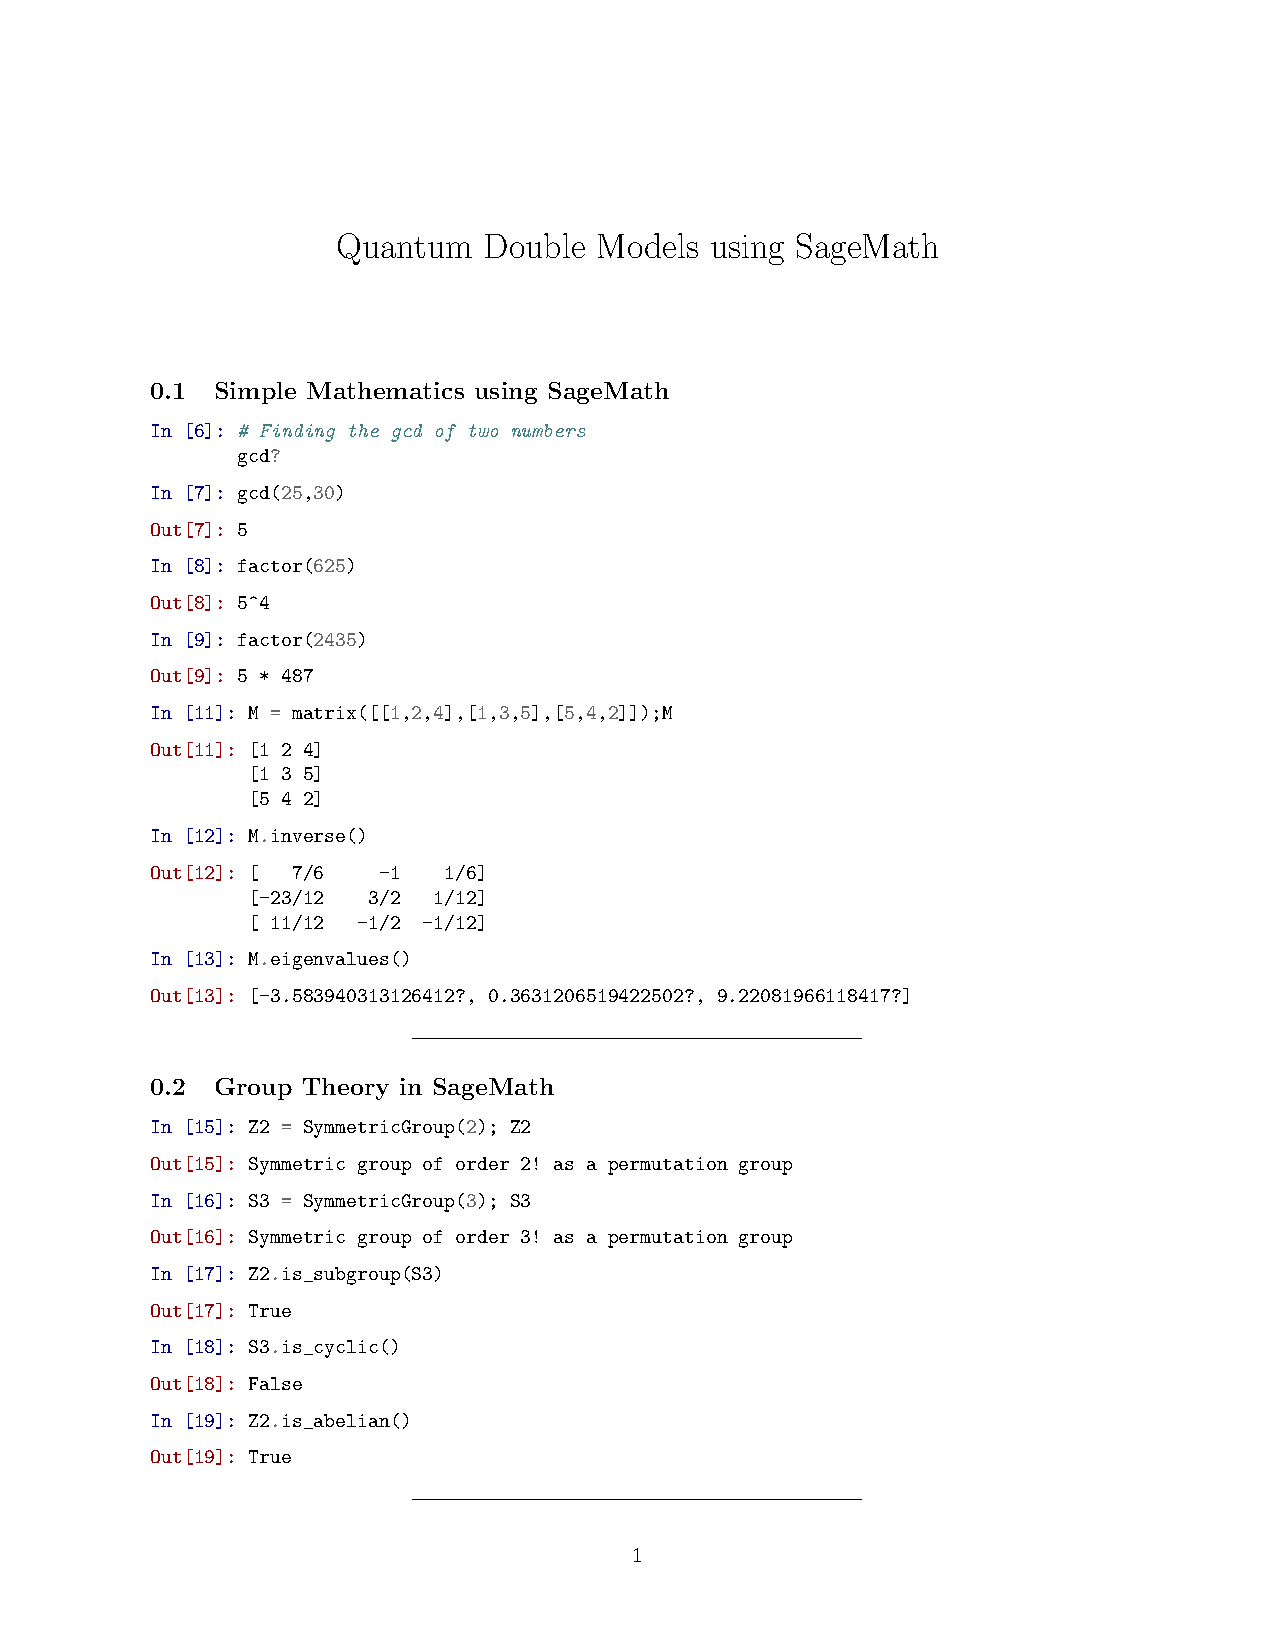
\includepdf[pages=-, offset=50 -50]{QDMSageMath.pdf}
%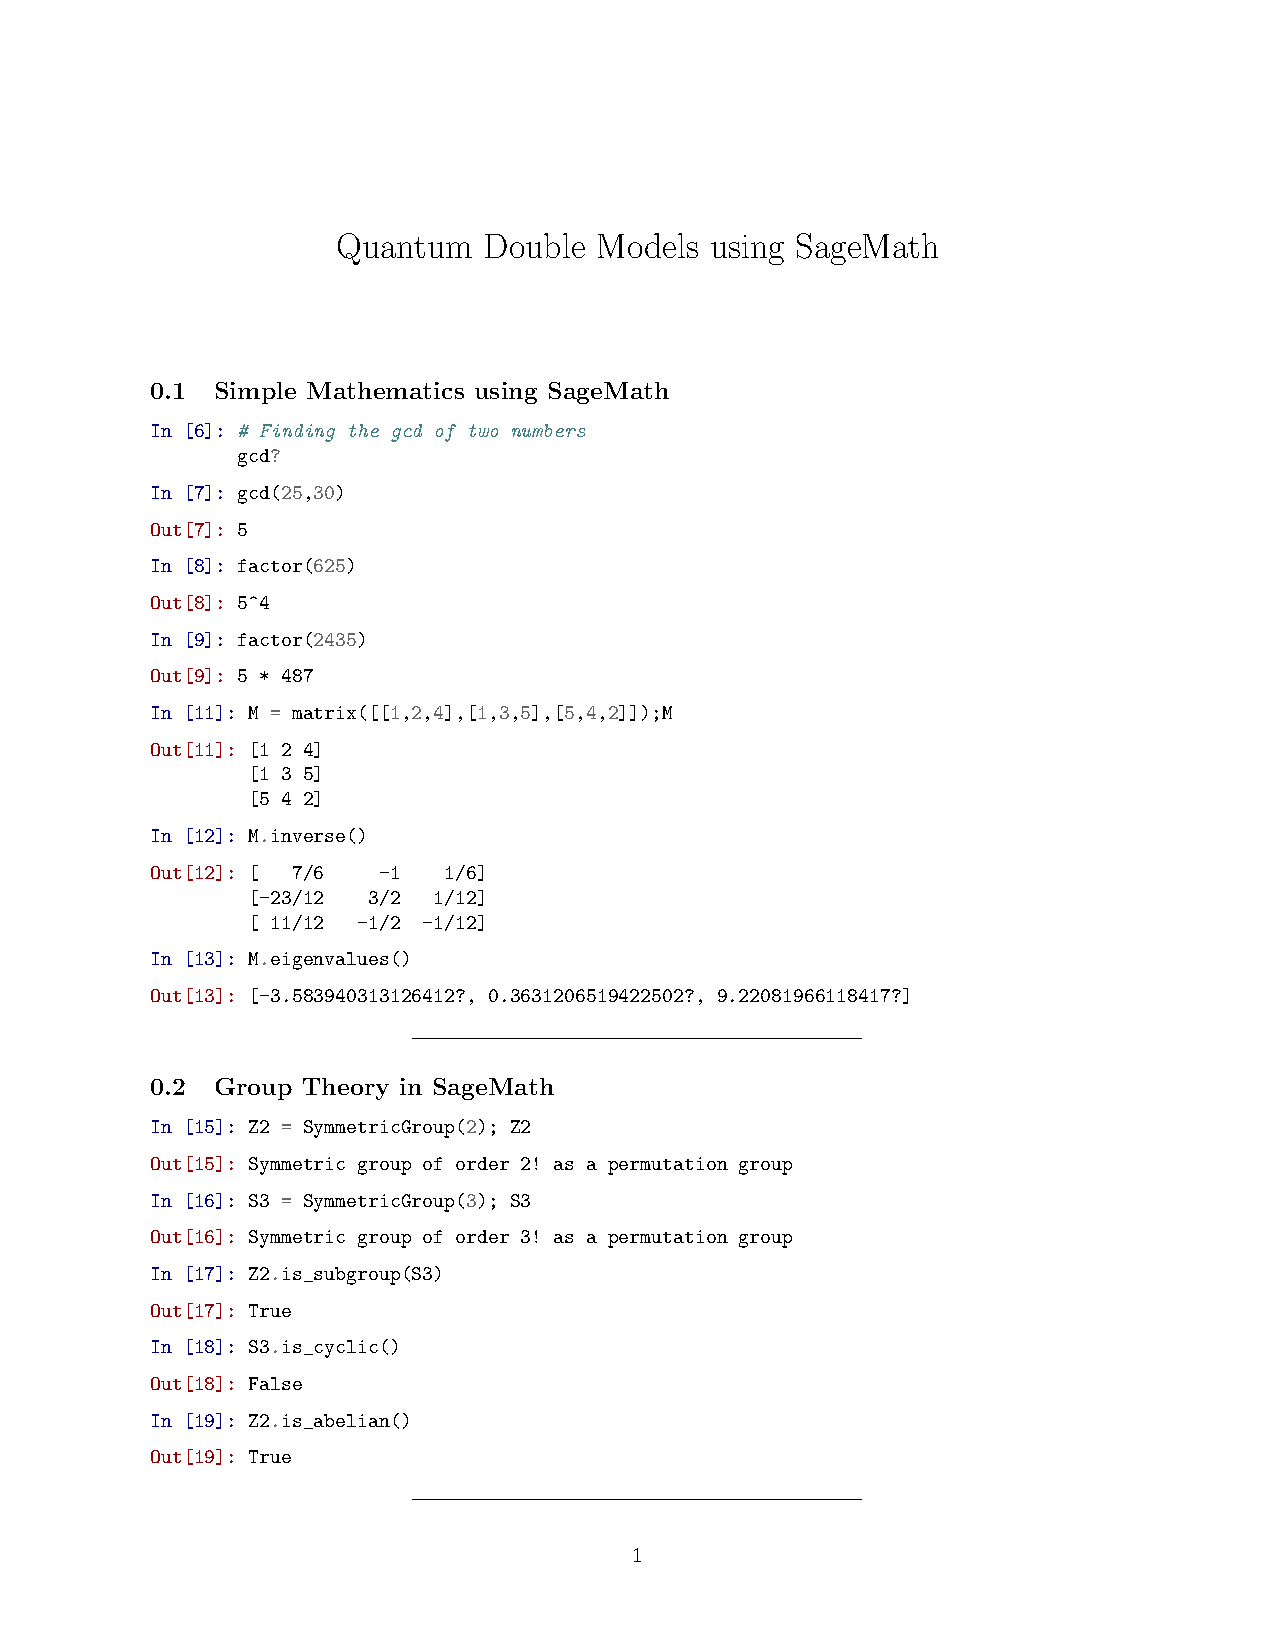
\includegraphics{QDMSageMath.pdf}
%\input{Appendices/AppendixB}
%\input{Appendices/AppendixC}

\addtocontents{toc}{\vspace{2em}} % Add a gap in the Contents, for aesthetics

\backmatter

%----------------------------------------------------------------------------------------
%	BIBLIOGRAPHY
%----------------------------------------------------------------------------------------

\label{Bibliography}

\lhead{\emph{Bibliography}} % Change the page header to say "Bibliography"

\bibliographystyle{unsrtnat} % Use the "unsrtnat" BibTeX style for formatting the Bibliography

\bibliography{Bibliography} % The references (bibliography) information are stored in the file named "Bibliography.bib"

\end{document}  